% !BIB TS-program = biber

\RequirePackage[l2tabu,orthodox]{nag}

% TODO: decide if one-sided/two-sided
%\documentclass[headsepline,footsepline,footinclude=false,fontsize=11pt,paper=a4,listof=totoc,bibliography=totoc,BCOR=12mm,DIV=12]{scrbook} % two-sided
\documentclass[headsepline,footsepline,footinclude=false,oneside,fontsize=11pt,paper=a4,listof=totoc,bibliography=totoc]{scrbook} % one-sided

\PassOptionsToPackage{table,svgnames,dvipsnames}{xcolor}

\usepackage[utf8]{inputenc}
\usepackage[T1]{fontenc}
\usepackage[sc]{mathpazo}
\usepackage[ngerman,american]{babel}
\usepackage[autostyle]{csquotes}
\usepackage[%
  backend=biber,
  url=false,
  style=numeric,
  maxnames=4,
  minnames=3,
  maxbibnames=99,
  giveninits,
  uniquename=init,
  sorting=none]{biblatex}
\usepackage{graphicx}
\usepackage{scrhack} % necessary for listings package
\usepackage{listings}
\usepackage{lstautogobble}
\usepackage{tikz}
\usepackage{pgfplots}
\usepackage{pgfplotstable}
\usepackage{booktabs}
\usepackage[final]{microtype}
\usepackage{caption}
\usepackage[printonlyused]{acronym}
\usepackage[hidelinks]{hyperref} % hidelinks removes colored boxes around references and links
\usepackage{physics}
\usepackage{qcircuit}
\AtBeginDocument{%
	\hypersetup{
		pdftitle=\getTitle,
		pdfauthor=\getAuthor,
	}
}
\usepackage{ifthen}

% for fachschaft_print.pdf
\makeatletter
\if@twoside{}
	\typeout{TUM-Dev LaTeX-Thesis-Template: twoside}
\else
	\typeout{TUM-Dev LaTeX-Thesis-Template: oneside}
\fi
\makeatother

\addto\extrasamerican{
	\def\lstnumberautorefname{Line}
	\def\chapterautorefname{Chapter}
	\def\sectionautorefname{Section}
	\def\subsectionautorefname{Subsection}
	\def\subsubsectionautorefname{Subsubsection}
}

\addto\extrasngerman{
	\def\lstnumberautorefname{Zeile}
}

% Themes
\ifthenelse{\equal{\detokenize{dark}}{\jobname}}{%
  % Dark theme
  \newcommand{\bg}{black} % background
  \newcommand{\fg}{white} % foreground
  \usepackage[pagecolor=\bg]{pagecolor}
  \color{\fg}
}{%
  % Light theme
  \newcommand{\bg}{white} % background
  \newcommand{\fg}{black} % foreground
}

\bibliography{bibliography}

\setkomafont{disposition}{\normalfont\bfseries} % use serif font for headings
\linespread{1.05} % adjust line spread for mathpazo font

% Add table of contents to PDF bookmarks
\BeforeTOCHead[toc]{{\cleardoublepage\pdfbookmark[0]{\contentsname}{toc}}}

% Define TUM corporate design colors
% Taken from http://portal.mytum.de/corporatedesign/index_print/vorlagen/index_farben
\definecolor{TUMBlue}{HTML}{0065BD}
\definecolor{TUMSecondaryBlue}{HTML}{005293}
\definecolor{TUMSecondaryBlue2}{HTML}{003359}
\definecolor{TUMBlack}{HTML}{000000}
\definecolor{TUMWhite}{HTML}{FFFFFF}
\definecolor{TUMDarkGray}{HTML}{333333}
\definecolor{TUMGray}{HTML}{808080}
\definecolor{TUMLightGray}{HTML}{CCCCC6}
\definecolor{TUMAccentGray}{HTML}{DAD7CB}
\definecolor{TUMAccentOrange}{HTML}{E37222}
\definecolor{TUMAccentGreen}{HTML}{A2AD00}
\definecolor{TUMAccentLightBlue}{HTML}{98C6EA}
\definecolor{TUMAccentBlue}{HTML}{64A0C8}

% Settings for pgfplots
\pgfplotsset{compat=newest}
\pgfplotsset{
  % For available color names, see http://www.latextemplates.com/svgnames-colors
  cycle list={TUMBlue\\TUMAccentOrange\\TUMAccentGreen\\TUMSecondaryBlue2\\TUMDarkGray\\},
}

% Settings for lstlistings
\lstset{%
  basicstyle=\ttfamily,
  columns=fullflexible,
  autogobble,
  keywordstyle=\bfseries\color{TUMBlue},
  stringstyle=\color{TUMAccentGreen},
  captionpos=b
}

\setlength\parindent{24pt}

\setcounter{secnumdepth}{3}

\newcommand*{\getUniversity}{Technische Universität München}
\newcommand*{\getFaculty}{Informatics}
\newcommand*{\getDegree}{Informatics}
\newcommand*{\getSchool}{Computation, Information and Technology}
\newcommand*{\getTitle}{Leveraging Noise in Quantum Machine Learning to Improve Model Robustness}
\newcommand*{\getTitleGer}{Nutzung von Rauschen beim Quantenmaschinellen Lernen zur Verbesserung der Modellrobustheit}
\newcommand*{\getAuthor}{Erick Ruben Quintanar Salas}
\newcommand*{\getDoctype}{Master's Thesis}
\newcommand*{\getSupervisor}{Prof.\ Dr.\ Claudia Eckert}
\newcommand*{\getAdvisor}{M. Sc. Pascal Debus / M. Sc. Kilian Tscharke}
\newcommand*{\getSubmissionDate}{October 31st, 2024}
\newcommand*{\getSubmissionLocation}{Munich}

\begin{document}

% Set page numbering to avoid "destination with the same identifier has been already used" warning for cover page.
% (see https://en.wikibooks.org/wiki/LaTeX/Hyperlinks#Problems_with_Links_and_Pages).
\pagenumbering{alph}
\begin{titlepage}
  % HACK for two-sided documents: ignore binding correction for cover page.
  % Adapted from Markus Kohm's KOMA-Script titlepage=firstiscover handling.
  % See http://mirrors.ctan.org/macros/latex/contrib/koma-script/scrkernel-title.dtx,
  % \maketitle macro.
  \oddsidemargin=\evensidemargin\relax
  \textwidth=\dimexpr\paperwidth-2\evensidemargin-2in\relax
  \hsize=\textwidth\relax

  \centering

  %\IfFileExists{logos/tum-\fg.pdf}{%
  %  \includegraphics[height=20mm]{logos/tum-\fg.pdf}
  %}{%
  %  \vspace*{20mm}
  %}

  \begin{tikzpicture}[y = -1cm, scale = .40]
    \draw (0, 0) -- (4, 0) -- (4, 4) -- (5, 4) -- (5, 0) -- (10, 0) --
          (10, 5) -- (9, 5) -- (9, 1) -- (8, 1) -- (8, 5) -- (7, 5) --
    (7, 1) -- (6, 1) -- (6, 5) -- (3, 5) -- (3, 1) -- (2, 1) --
    (2, 5) -- (1, 5) -- (1, 1) -- (0, 1) -- cycle
    %[line width = 0pt, draw = white, fill = tumblue];
    [fill = TUMBlue, line width = 0pt, draw = white];
  \end{tikzpicture}

  \vspace{5mm}
  {\huge\MakeUppercase{School of \getSchool{} --- \getFaculty{}} \par}

  \vspace{5mm}
  {\large\MakeUppercase{\getUniversity{}} \par}

  \vspace{25mm}
  {\Large \getDoctype{} in \getDegree{} \par}

  \vspace{10mm}
  {\huge\bfseries \getTitle{} \par}

  \vspace{10mm}
  {\LARGE \getAuthor{}}

  \vspace{30mm}
  \begin{tikzpicture}
    \draw (0, 0) arc (95:445:1cm) [ultra thick, draw = TUMBlue];
    \draw (0.09, 0.2) -- (0.09, -1.8) [very thick, draw = TUMBlue];
  \end{tikzpicture}

  \IfFileExists{logos/faculty-\fg.pdf}{%
    \vfill{}
    \includegraphics[height=20mm]{logos/faculty-\fg.pdf}
  }{}
\end{titlepage}


\frontmatter{}

\begin{titlepage}
  \centering

  \IfFileExists{logos/tum-\fg.pdf}{%
    \includegraphics[height=20mm]{logos/tum-\fg.pdf}
  }{%
    \vspace*{20mm}
  }

  \vspace{5mm}
  {\huge\MakeUppercase{School of \getSchool{} --- \getFaculty{}} \par}

  \vspace{5mm}
  {\large\MakeUppercase{\getUniversity{}} \par}

  \vspace{20mm}
  {\Large \getDoctype{} in \getDegree{} \par}

  \vspace{15mm}
  {\huge\bfseries \getTitle{} \par}

  \vspace{10mm}
  {\huge\bfseries \foreignlanguage{ngerman}{\getTitleGer{}} \par}

  \vspace{10mm}
  \begin{tabular}{l l}
    Author:          & \getAuthor{}         \\
    Supervisor:      & \getSupervisor{}     \\
    Advisors:         & \getAdvisor{}        \\
    Submission Date: & \getSubmissionDate{} \\
  \end{tabular}

  \IfFileExists{logos/faculty-\fg.pdf}{%
    \vfill{}
    \includegraphics[height=20mm]{logos/faculty-\fg.pdf}
  }{}
\end{titlepage}

\input{pages/disclaimer}
\addcontentsline{toc}{chapter}{Acknowledgments}
\thispagestyle{empty}

\vspace*{20mm}

\begin{center}
    {\usekomafont{sectioning}\usekomafont{section} Acknowledgments}
\end{center}

\vspace{10mm}

I want to thank first my supervisors Kilian Tscharke and Pascal Debus,
without their guidance and help this thesis would not have been possible. \
I also want to thank my friends and family for their unconditional
love and support. Fatma, María, Rubén, Joanna, Chuy and Oscar, I hope one
day I will be able to repay you everything you have given me. Additionally,
I want to thank Nicola Franco and David Winderl for sharing their expertise
on quantum machine learning. Last but not least, I want to thank Prof. Dr.
Claudia Eckert for the giving me the opportunity to work on this thesis
in a very new and exciting field. 

\cleardoublepage{}

\chapter{\abstractname}

This thesis explores the potential of utilizing quantum noise in \acl{qml}
models to enhance robustness against adversarial attacks. Quantum noise,
typically seen as a challenge in quantum computing, is applied here with
the hypothesis that it may improve model resilience. This thesis employs a
\acl{vqa} to evaluate the effects of different types and strengths of
quantum noise on the robustness of \ac{qml} models under adversarial
conditions created by \acl{fgsm} and \acl{pgd} attacks. The work examines
both noisy and noiseless models, revealing four main scenarios of
adversarial performance across various noise combinations. \

Interestingly, results indicate that while some noisy models achieve
higher adversarial accuracy at specific attack strengths, no
direct linear relationship exists between noise probability and
model robustness. This lack of a straightforward correlation suggests
that certain noise configurations might indeed offer resilience advantages,
although the outcomes vary based on attack type and dataset. Additionally,
quantum noise utilized during the training phase does not alter the model's
final state, as the weights are adapted to noise conditions in
training yet evaluated noiselessly. This distinction offers
insights into how noise affects parameter adjustments rather
than the final classification states, proposing a nuanced
understanding of robustness in noisy QML environments. \

This thesis contributes to the field of quantum adversarial machine
learning by demonstrating that quantum noise may serve as a resource
for improving \acl{qml} model resilience under adversarial attacks. 
Potentially, this thesis enables the development of \ac{qml}
architectures that inherently integrate quantum noise for
robustness purposes without sacrificing model performance on
non-adversarial samples. \
\microtypesetup{protrusion=false}
\tableofcontents{}
\microtypesetup{protrusion=true}

\mainmatter{}

\chapter{Introduction}\label{chapter:introduction} \

In recent years the interest on techniques to utilize quantum mechanics has been rising.
One of the many applications is quantum computing, where devices based on the laws
of quantum theory are exploited to process information~\cite{national_academies_of_sciences_engineering_and_medicine_quantum_2019}.
Although current classical computers have become very powerful, they still struggle to
process many applications that quantum computers can in theory easily solve. \

Many quantum algorithms for quantum computers have been proposed that highly
outperform a classical computer with the best known algorithms~\cite{shor_polynomial-time_1997, van_dam_quantum_2006, hallgren_polynomial-time_2007}.
These quantum algorithms solve in polynomial time problems that quickly become
intractable to solve in a classical computer, as they normally grow exponentially.
The most famous algorithm is Shor's algorithm~\cite{shor_polynomial-time_1997}, which can find the prime factors
of an integer. It is of special interest because if quantum devices
were able to execute it, the current confidentiality and integrity guarantees
that the RSA~\cite{rivest_method_1978} cryptographic mechanism offers would be violated. \

\section{Motivation} \

Even though the previously mentioned quantum algorithms would surpass the performance
of the best classical ones, they still can not be executed on current quantum
computers due to noise~\cite{preskill_quantum_2018}. This noise occurs because
current quantum devices are not completely isolated from the environment and every
time we perform an operation on them we introduce a disturbance. This type of device
is known as \ac{nisq}, meaning that there will be significant noise when operating
the quantum device. \

In order to reduce the influence of noise in \ac{nisq} devices, either the precision
in which quantum computers can be manipulated has to improve or error-correcting
codes have to be implemented~\cite{shor_quantum_nodate}. Currently both techniques are
being heavily researched and in conjunction will lead to the next generation of
quantum devices, namely fault-tolerant quantum computers. \

A technology that right now has gained a bigger presence in our society is \ac{ml}.
There have been many important breakthroughs for \ac{ml} in the past few years, with
uses in natural language processing, computer vision, anomaly detection, and many
more fields~\cite{bommasani_opportunities_2022}. Nowadays \ac{ml} has a big impact
in society, and even though it depicts big opportunities for improvement in
society it also represents significant risks. \

Quantum computing and \ac{ml} are information processing techniques that have
improved significantly in recent years. This lead to the natural desire of
harnessing the advantages of both and to the emergence of a new field of study
denominated \ac{qml}~\cite{schuld_machine_2021}. \ac{qml} explores several ideas
like whether quantum devices are better at \ac{ml} than classical computers or
if quantum information adds new data that affects how machines recognize patterns. \

Returning to the possible risks that \ac{ml} might encounter, several attacks have
been developed to force a \ac{ml} model to missclassify an input~\cite{szegedy_intriguing_2014}.
These attacks are denominated adversarial attacks and are based on crafting specific
input data that has been slightly modified to cause the model to erroneously classify
the input. These small modifications are imperceptible for humans. At the beginning,
when the first adversarial attacks were developed, they needed to know the
architecture of the model to be able to fool it. Nevertheless, it was proved
that adversarial attacks are transferable between models with the same use
case, without knowing the architecture of the model or the dataset it was
trained on~\cite{papernot_transferability_2016}. \

Adversarial training was developed in order to defend \ac{ml} models against
adversarial attacks~\cite{goodfellow_explaining_2015, szegedy_intriguing_2014}.
Adversarial training consists of including adversarial samples into the training
of the \ac{ml} model to better generalize its classification. This mechanism
has a tradeoff, in which the accuracy of the model lowers, while increasing the
resilience to adversarial attacks~\cite{kurakin_adversarial_2017}. \

In classical \ac{ml}, noise in training has been shown to improve generalization
performance and local optima avoidance~\cite{ciliberto_quantum_2018}. This
property from noise is particularly interesting in \ac{nisq} devices, as their
inherent noise might be able to improve \ac{qml} performance, accuracy and
resilience against adversarial attacks. \

\section{Research Goals} \

The main goal of this thesis is to investigate the effects of quantum noise
on the resilience of \ac{qml} models against adversarial
attacks. To achieve this we set four intermediate goals that build
upon each other to fulfill the main goal. These goals are: \

\begin{enumerate}
    \item \textbf{Train noiseless \ac{qml} models on different datasets:}
            We choose different datasets to train several \ac{qml} models.
            Selecting distinct datasets, each with increasing amount of
            features, will test the baseline performance of the \ac{qml}
            models and set a benchmark for the upcoming noisy models. \
    \item \textbf{Train noisy \ac{qml} models on different datasets:} Once
            the baseline \ac{qml} model accuracy for the different datasets
            has been established, we then train more \ac{qml} models that
            suffer from quantum noise. We choose six different types of
            noise models and for each type we modify the magnitude of the
            noise with five different values. This allows us not only
            to compare noiseless and noisy \ac{qml} models performance,
            but also to observe the impact of quantum noise on the models'
            accuracy. \
    \item \textbf{Perform adversarial attacks on noiseless \ac{qml} models:}
            We perform two different adversarial attacks on the noiseless
            \ac{qml} models for the different datasets. This will allow
            us to obtain the adversarial examples to further evaluate the
            previously trained noisy models. Two differet adversarial
            techniques with five different attack strenghts are utilized
            to validate the possible effects of quantum noise as a defense
            against adversarial attacks. \
    \item \textbf{Evaluate noisy \ac{qml} models with adversarial samples:}
            Finally, with the adversarial examples obtained from the noiseless
            models, we test all the noisy \ac{qml} models with the different
            constelations of noise magnitude. We cover different types of noise
            with different noise magnitudes as well as different attack techniques
            with increasing attack strenght. This will enable us to verify
            any possible effect caused by quantum noise on \ac{qml} model robustness
            against adversarial attacks. \
  \end{enumerate} \

\section{Outline} \

This thesis is structured as follows. In Chapter~\ref{chapter:background}
we will introduce the required quantum computing, quantum noise, \ac{qml},
and \ac{aml} concepts important for this thesis. Furthermore, in Chapter
~\ref{chapter:design} we will present the design decisions (and their
justification) taken to implement the experiments aimed at investigating
the research questions. Moreover, in Chapter~\ref{chapter:implementation}
we describe the procedure that the tests follow to provide information
about the research goals. Additionally, in Chapter~\ref{chapter:results}
we provide the results of the conducted experiments and discuss the observed
findings. Finally, a summary of the thesis and some suggestions on what
can be further researched are given in Chapter~\ref{chapter:summary} and
Chapter~\ref{chapter:future_work} respectively.\
\chapter{Theoretical Background}\label{chapter:background} \

In Chapter~\ref{chapter:background} we will introduce the
background information that is required to understand
the main ideas of this thesis. First we introduce
the basic concepts of quantum computing. Then we will
describe advanced concepts regarding quantum noise. We
assume some baseline \ac{ml} knowledge, however, we
will provide an outlook into \ac{qml}. Finally, we
present several types of adversarial machine learning
and adversarial training as a defense mechanism. \

\section{Fundamentals of Quantum Computing} \

% TODO: Most concepts are presented in a simpliflied way.
%       Say most info can be found in books. if not fully
%       understood.
%       Introduce all the written concepts, linked with their references

\subsection{Qubit}\label{subsection:qubit} \

The basic computing unit in quantum computing is the
\textit{qubit}~\cite{schumacher_quantum_1995}. Similar to the classical
bit, a qubit also has a state. While a bit has either a
\textit{0} or \textit{1} state, the qubit can have
many more states. The quantum equivalent to the classical
bit states would be \(\ket{0}\) and \(\ket{1}\) (spoken as \textit{ket}) in Dirac
notation~\cite{dirac_new_1939} and they represent the orthonormal computational
basis states in Equation~\ref{eq:qubit_bases}. \

\begin{equation}\label{eq:qubit_bases}
    \ket{0} = \begin{pmatrix}
                1 \\ 0
              \end{pmatrix} \qquad \qquad
    \ket{1} = \begin{pmatrix}
                0 \\ 1
              \end{pmatrix}
\end{equation} \

The complementing element to Dirac's notation is the \textit{bra}:
\(\bra{0}\) and \(\bra{1}\). The \textit{bra} is the conjugate transposed
vector from a \textit{ket}. The outer product of two vectors \(u\) and
\(v\) in dirac notation is written as \(\ketbra{u}{v}\). While the inner
product of the same vectors is expressed as \(\braket{u}{v}\). \

What makes the qubit different and more capable than
the classical bit is that it can also have different states
created by a linear combination or \textit{superposition} from
its basis states. The linear combination in Equation
~\ref{eq:qubit_superposition} is the complete representation
of a qubit, where \(\alpha\) and \(\beta\) are two complex numbers that
are denominated \textit{probability amplitudes}.
The values \(\alpha\) and \(\beta\) represent a distribution, in which
with probability \(|\alpha|^2\) we will observe a \textit{0}
value and with probability \(|\beta|^2\) we will observe a
\textit{1} value. This distribution is determined by the
Born rule~\cite{born_quantenmechanik_1926} and states that \(|\alpha|^2 + |\beta|^2 \stackrel{!}{=} 1\).
The Born rule thus implies that a qubit state is a unitary vector in
a two-dimensional complex vector space. Although the
probability amplitudes can take on any complex value as long
as they fulfill the Born rule, when we perform a measurement
on the qubit it \textit{collapses} to one of the two basis
states. \

\begin{equation}\label{eq:qubit_superposition}
  \ket{\psi} = \alpha\ket{0} + \beta\ket{1}
\end{equation} \

In the real physical world qubits can be implemented by
several different small particles. However, the mathematical
qubit abstraction helps establish a baseline computing unit
for quantum computing independent of which particle it is
being represented by~\cite{nielsen_quantum_2010}. While in this perfect
mathematical description noise does not occur, there are
different mechanisms to represent the noise that quantum
computers suffer from, namely the density operator that will
be introduced in Subsection~\ref{subsection:density_operator}. \

\subsection{Bloch Sphere}\label{subsection:bloch} \

The qubit state from Equation~\ref{eq:qubit_superposition} can be
rewritten into Equation~\ref{eq:qubit_global_phase}, where \(e\)
is the Euler number, \(i\) is the imaginary number, and \(\gamma\),
\(\varphi\), and \(\theta\) are real numbers. \

\begin{equation}\label{eq:qubit_global_phase}
  \ket{\psi} = e^{i\gamma} \left( \cos{\frac{\theta}{2}}\ket{0} + e^{i\varphi}\sin{\frac{\theta}{2}}\beta\ket{1} \right)
\end{equation} \

Because for a single qubit the global phase \(e^{i\gamma}\) has no
observable effects, we can omit it and write the state of a qubit as: \

\begin{equation}\label{eq:qubit_bloch}
  \ket{\psi} = \cos{\frac{\theta}{2}}\ket{0} + e^{i\varphi}\sin{\frac{\theta}{2}}\beta\ket{1}
\end{equation} \

where \(\theta\) and \(\varphi\) determine a point in the Bloch
sphere~\cite{bloch_nuclear_1946}. The Bloch sphere (Fig.~\ref{fig:bloch_sphere})
is a helpful visual representation for understanding the state of a
qubit. In Section~\ref{section:noise} this representation will be
utilized to show the effects of quantum noise on a quantum state. It
can also be used to visualize the effect of the operations performed
on quantum states, these operations are called \textit{gates} and 
they will be introduced in Subsection~\ref{subsection:gates}. \

\begin{figure}[ht]
  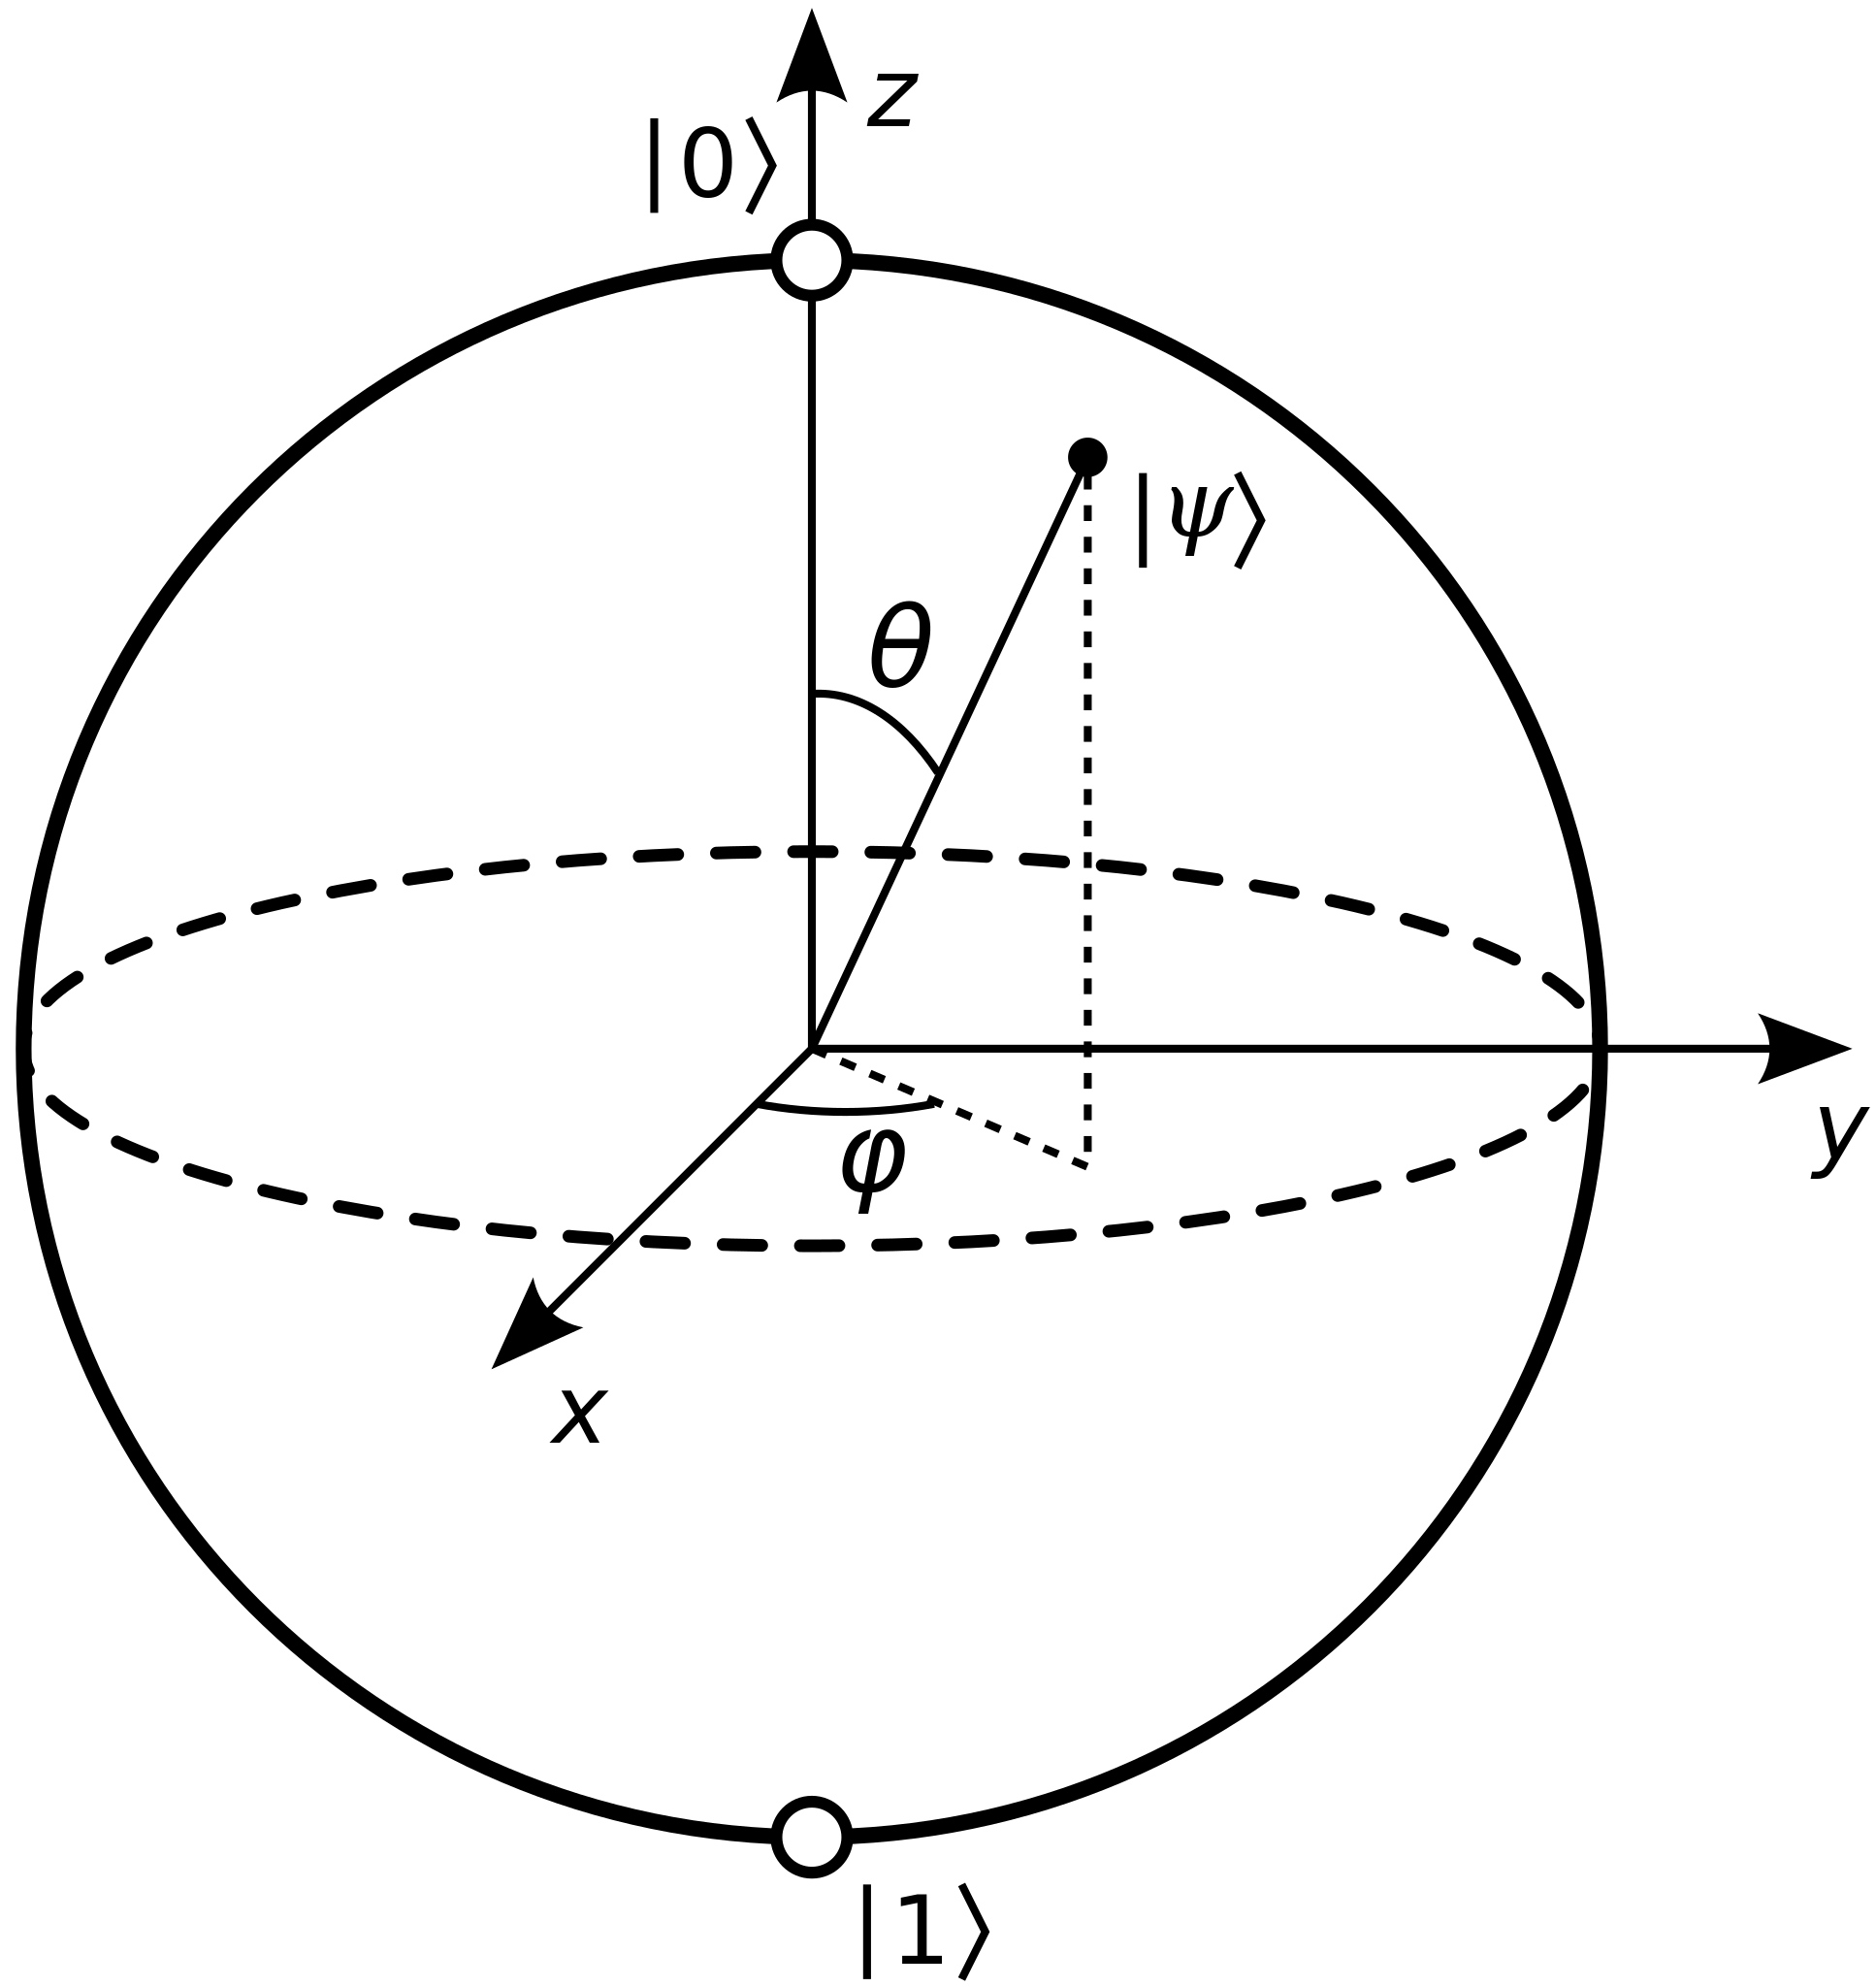
\includegraphics[scale=0.1]{figures/Bloch_sphere.png}
  \centering
  \caption{Bloch sphere representation of a qubit. Image taken from \href{https://commons.wikimedia.org/wiki/File:Bloch_Sphere.svg}{Wikimedia Commons} under the \href{https://en.wikipedia.org/wiki/Creative_Commons}{Creative Commons Attribution-Share Alike 3.0 Unported license}.}
~\label{fig:bloch_sphere}
\end{figure} \

\subsection{Multiple qubits} \

To describe multiple qubits we utilize the fundamentals presented in
Subsection~\ref{subsection:qubit} and expand them. For two qubits
\(\ket{00}, \ket{01}, \ket{10}\), and \(\ket{11}\) are the computational basis.
A general representation for a two qubit system can be found in 
Equation~\ref{eq:two_qubits}, where all the probability amplitudes must
follow the Born rule. \ 

\begin{equation}\label{eq:two_qubits}
  \ket{\psi} = \alpha_{00}\ket{00} + \alpha_{01}\ket{01} + \alpha_{10}\ket{10} + \alpha_{11}\ket{11}
\end{equation} \

Due to the Born rule the measurement results for
\(x = \left\{00, 01, 10, 11\right\}\) follow the probability
distribution determined by \(|\alpha_{x}|^2\). Similar to a
single qubit, once a measurement on both qubits is performed,
the state of the qubits will collapse to the measured computational
basis. Nevertheless, with multiple qubits we are able to perform
measurements on a subset of qubits. In the case of a two-qubit
system, measuring the first qubit will collapse its value. However,
the second's qubit state will remain. In the case of Eq.~\ref{eq:two_qubits},
if \textit{0} was measured in the first qubit, the amplitudes \(\alpha_{10}\)
and \(\alpha_{11}\) would disappear from the state as they are no longer
possible. Furthermore, the remaining amplitudes must be normalized,
such as in Eq.~\ref{eq:measure_first}, to fulfill the normalization
restriction.  \

\begin{equation}\label{eq:measure_first}
  \ket{\psi'} = \frac{\alpha_{00}\ket{00} + \alpha_{01}\ket{01}}
                    {\sqrt{|\alpha_{00}|^2 + |\alpha_{01}|^2}}
\end{equation} \

In Equation~\ref*{eq:multiple_qubits} we can find a general representation of
a set of \textit{n} qubits. For a system composed by \textit{n} qubits there are \(2^n\)
amplitudes. If we tried to simulate a quantum system with \(n = 50\), assuming
that complex numbers require 8 bytes to be stored~\cite{harris_array_2020}, a classical computer would need
approximately 9000 terabytes to store the generated quantum state. This simple calculation
shows the reason why quantum computers are so promising and also why classical computers
are not able to process quantum information efficiently. \
% (2**50)*8 = 9007199254740992
% https://docs.scipy.org/doc/numpy-1.17.0/user/basics.types.html

\begin{equation}\label{eq:multiple_qubits}
  \ket{\psi} = \alpha_{00}\ket{0\cdots0} + \cdots + \alpha_{2^{n-1}}\ket{1\cdots1}
\end{equation} \

\subsection{Quantum Gates}\label{subsection:gates}\

Once that quantum states have been defined, performing operations
on them is the next step to understand how quantum computing works.
These operations are denominated \textit{quantum gates} and they
modify the quantum state according to its properties. A quantum gate
can be represented as a matrix that fulfills one single property,
namely that it is a unitary matrix. In Equation~\ref{eq:unitary} we
can observe that a unitary matrix is one which when multiplied by its
own transpose conjugate is equal to the identity matrix.

\begin{equation}\label{eq:unitary}
  UU^{\dag} = I \qquad \qquad
  \ket{\psi} \xrightarrow{U} U\ket{\psi} = \ket{\psi'}
\end{equation}

This property is required because when a quantum gate is used on a
quantum state (Eq.~\ref{eq:unitary}), the resulting quantum state has to be a valid normalized
quantum state. By being a unitary matrix, this effect is achieved.
There are infinitely many unitary matrices, however, there are some
of specific importance. The most important single-qubit quantum
gates will be introduced in Subsection~\ref{subsubsection:single_qubit},
while the most significant multiple-qubits gates will be presented
in Subsection~\ref{subsubsection:multiple_qubit} \

\subsubsection{Single-Qubit Gates}\label{subsubsection:single_qubit} \

Single-Qubit gates can be described by a two by two unitary matrix. The
first three quantum gates introduced are described by the Pauli matrices.
They are defined as the X, Y and Z gates because each matrix represents
a \(\pi\) rotation around the Bloch sphere in their respective axis. \

\paragraph{X Gate} \

The X gate's matrix and its gate representations can be found in
Equation~\ref{eq:pauli_x}. In classical computing, the X gate is
conceptually equivalent to the NOT gate, thus it
is also known as a quantum NOT gate. \

\begin{equation}\label{eq:pauli_x}
  X = \begin{pmatrix}
        0 & 1 \\
        1 & 0
      \end{pmatrix} \qquad \qquad
  \Qcircuit @C=1em @R=1em {
    & \gate{X} & \qw
  } \qquad
  \Qcircuit @C=1em @R=1em {
    & \targ & \qw
  }
\end{equation} \

In Equation~\ref{eq:pauli_x_basis} we can see the effect of the X
gate, where the computational basis states are flipped. This phenomena
is known as a \textit{bit flip}. \

\begin{equation}\label{eq:pauli_x_basis}
  X\ket{0} = \begin{pmatrix}
               0 & 1 \\
               1 & 0
             \end{pmatrix}
             \begin{pmatrix} 1 \\ 0 \end{pmatrix} = 
             \begin{pmatrix} 0 \\ 1 \end{pmatrix} =
             \ket{1}, \qquad
  X\ket{1} = \begin{pmatrix}
              0 & 1 \\
              1 & 0
            \end{pmatrix}
            \begin{pmatrix} 0 \\ 1 \end{pmatrix} = 
            \begin{pmatrix} 1 \\ 0 \end{pmatrix} =
            \ket{0}
\end{equation} \

\paragraph{Z Gate} \

Unlike the X gate, there is no conceptually equivalent
gate for the Z gate in classical computing. In Equation~\ref{eq:pauli_z}
we can observe the matrix and symbol representation of the Z gate. \

\begin{equation}\label{eq:pauli_z}
  Z = \begin{pmatrix}
        1 & 0 \\
        0 & -1
      \end{pmatrix} \qquad \qquad
  \Qcircuit @C=1em @R=1em {
    & \gate{Z} & \qw
  }
\end{equation} \

The effects of the Z gate can be found in Equation~\ref{eq:pauli_z_basis}.
We can observe that the \(\ket{0}\) state remains unmodified while
the \(\ket{1}\) state is negative after the operation. This phenomena
is known as a \textit{phase flip}. \

\begin{equation}\label{eq:pauli_z_basis}
  Z\ket{0} = \begin{pmatrix}
               1 & 0 \\
               0 & -1
             \end{pmatrix}
             \begin{pmatrix} 1 \\ 0 \end{pmatrix} = 
             \begin{pmatrix} 0 \\ 1 \end{pmatrix} =
             \ket{0}, \qquad
  Z\ket{1} = \begin{pmatrix}
               1 & 0 \\
               0 & -1
            \end{pmatrix}
            \begin{pmatrix} 0 \\ 1 \end{pmatrix} = 
            \begin{pmatrix} 1 \\ 0 \end{pmatrix} =
            -\ket{1}
\end{equation} \

\paragraph{Y Gate} \

The Y gate also doesn't have a conceptually equivalent gate
in classical computing. More interestingly the Y gate can be described
by the product of the X and Z matrix up to a global phase. The matrix
and symbol representation of the Y gate can be found in
Equation~\ref{eq:pauli_y}. \

\begin{equation}\label{eq:pauli_y}
  Y = \begin{pmatrix}
        0 & -i \\
        i & 0
      \end{pmatrix} \qquad \qquad
  \Qcircuit @C=1em @R=1em {
    & \gate{Y} & \qw
  }
\end{equation} \

In Equation~\ref{eq:pauli_y_basis} we can see how the Y gate
modifies the computational basis states. In it we can observe that
a bit flip and a phase flip have been executed, while \(i\) has been
added as a global phase. \

\begin{equation}\label{eq:pauli_y_basis}
  Y\ket{0} = \begin{pmatrix}
               0 & -i \\
               i & 0
             \end{pmatrix}
             \begin{pmatrix} 1 \\ 0 \end{pmatrix} = 
             \begin{pmatrix} 0 \\ 1 \end{pmatrix} =
             i\ket{1}, \qquad
  Y\ket{1} = \begin{pmatrix}
               0 & -i \\
               i & 0
            \end{pmatrix}
            \begin{pmatrix} 0 \\ 1 \end{pmatrix} = 
            \begin{pmatrix} 1 \\ 0 \end{pmatrix} =
            -i\ket{0}
\end{equation} \

As a complement to the Pauli gates, there are gates that
perform a specific \(\theta\) rotation around each axis of the
Bloch sphere. They are known as \(RX\left(\theta\right)\),
\(RY\left(\theta\right)\) and \(RZ\left(\theta\right)\). \

% MAYBE: Expand the RXYZ gates as they can become important for
% parametrized ansatzs. schuld 104
% MAYBE: Expand on the general rotation gate RZ RY RZ

\paragraph{Hadamard Gate} \

The Hadamard gate is one of the most useful single-qubit gates.
It will be later used in Subsection~\ref{subsubsection:entanglement}
to create \textit{entanglement} between two different qubits. \

\begin{equation}\label{eq:hadamard}
  H = \frac{1}{\sqrt{2}} 
      \begin{pmatrix}
        1 & 1 \\
        1 & -1
      \end{pmatrix} \qquad \qquad
  \Qcircuit @C=1em @R=1em {
    & \gate{H} & \qw
  }
\end{equation} \

The effects of the Hadamard gate can be observed in
Equation~\ref{eq:hadamard_basis}. The resulting states from applying
the Hadamard gate to the computational basis are denominated
\(\ket{+}\) and \(\ket{-}\) respectively and they represent
a superposition with equal probability for both computational 
basis to be measured. \

\begin{equation}\label{eq:hadamard_basis}
  H\ket{0} = \frac{1}{\sqrt{2}} \left( \ket{0} + \ket{1} \right) = \ket{+} \qquad
  H\ket{1} = \frac{1}{\sqrt{2}} \left( \ket{0} - \ket{1} \right) = \ket{-}
\end{equation} \

Another interesting property of the previously mentioned single-qubit
gates is that all of them are involutory. An involutory matrix is a
square matrix that is its own inverse. This implies that performing
twice the same gate will not modify the quantum state as the identity
transformation would have been applied. \

% MAYBE: Add S and T gates

\subsubsection{Multiple-Qubits Gates}\label{subsubsection:multiple_qubit} \

Multiple-Qubits gates are not that different from single-qubit gates,
they still have to be unitary. Nevertheless, depending on the qubits
that the gate is trying to modify, the size of the matrix will change.
Formally, if a gate is applying a transformation to \(n\) qubits, then
the dimensions of the gate's matrix \(M \in \mathbb{C}^{2^n \times 2^n}\).
Therefore, if \(n = 2\) then \(M\) would have the size
\(\mathbb{C}^{4 \times 4}\). \

\paragraph{Controlled NOT Gate} \

The~\ac{cnot} gate is a two-qubit quantum gate. It has a
\textit{control} qubit and a \textit{target} qubit. In
Equation~\ref{eq:cnot} we can observe the matrix and
symbol representation where the first qubit is the control
qubit and the second is the target qubit. \

\begin{equation}\label{eq:cnot}
  CNOT = \begin{pmatrix}
          1 & 0 & 0 & 0 \\
          0 & 1 & 0 & 0 \\
          0 & 0 & 0 & 1 \\
          0 & 0 & 1 & 0 \\
        \end{pmatrix} \qquad \qquad
  \Qcircuit @C=1em @R=1em {
      & \ctrl{1} & \qw \\
      & \targ & \qw \\
  } \qquad \qquad
  \begin{matrix}
    CNOT\ket{00} = \ket{00} \\
    CNOT\ket{01} = \ket{01} \\
    CNOT\ket{10} = \ket{11} \\
    CNOT\ket{11} = \ket{10} \\
  \end{matrix}
\end{equation} \

The effects of the \ac{cnot} gate can be seen in Equation~\ref{eq:cnot},
where depending on the value of the control qubit, a NOT gate will be
applied on the target wire. This can also be represented as
\(\ket{A,B}\rightarrow\ket{A,B\oplus A}\) performing an XOR between
the control and target qubits and storing the value in the second qubit. \

Regarding the~\ac{cnot} matrix in Equation~\ref{eq:cnot}, an intuiton
can be gained regarding the columns of the matrix, the computational
basis, and the effects of the gate. The ordering of the columns each
represent the input state with regards to the computational basis.
The first column represents \(\ket{00}\), the second column \(\ket{01}\),
the third column \(\ket{10}\) and so on. Moreover, the values that the vectors
represent in each column are associated with the output values after the gate
has been applied, e.g. \(\begin{pmatrix}1&0&0&0\end{pmatrix}^\top= \ket{00}\),
\(\begin{pmatrix}0&1&0&0\end{pmatrix}^\top= \ket{01}\),
\(\begin{pmatrix}0&0&1&0\end{pmatrix}^\top= \ket{10}\), etc. \

We can observe this phenomena between the third and fourth column in
Eq.~\ref{eq:cnot}, where the columns and values swap. Also this
intuiton helps us construct the matrix from the~\ac{cnot} gate when the
control and the target qubits have been inverted. In  Equation~\ref{eq:cnot_inverted}
we construct the matrix from the effects the CNOT gate would have in
the different computation basis states. \

\begin{equation}\label{eq:cnot_inverted}
  \begin{matrix}
    CNOT\ket{00} = \ket{00} \\
    CNOT\ket{01} = \ket{11} \\
    CNOT\ket{10} = \ket{10} \\
    CNOT\ket{11} = \ket{01} \\
  \end{matrix} \qquad \qquad
  \Qcircuit @C=1em @R=1em {
      & \targ & \qw \\
      & \ctrl{-1} & \qw \\
  } \qquad \qquad
  CNOT_2 = \begin{pmatrix}
    1 & 0 & 0 & 0 \\
    0 & 0 & 0 & 1 \\
    0 & 0 & 1 & 0 \\
    0 & 1 & 0 & 0 \\
  \end{pmatrix}
\end{equation} \

\paragraph{SWAP gate} \

The SWAP gate's effect are introduced in Equation~\ref{eq:swap}. It shows
that the value of the first qubit is swapped with the value of the
second value. Therefore, the gate will only have an effect if the qubits'
values are different. \

\begin{equation}\label{eq:swap}
  SWAP = \begin{pmatrix}
          1 & 0 & 0 & 0 \\
          0 & 0 & 1 & 0 \\
          0 & 1 & 0 & 0 \\
          0 & 0 & 0 & 1 \\
        \end{pmatrix} \qquad \qquad
  \Qcircuit @C=1em @R=1em {
    & \qswap & \qw \\
    & \qswap \qwx & \qw \\
  } \qquad \qquad
  \begin{matrix}
    SWAP\ket{00} = \ket{00} \\
    SWAP\ket{01} = \ket{10} \\
    SWAP\ket{10} = \ket{01} \\
    SWAP\ket{11} = \ket{11} \\
  \end{matrix}
\end{equation} \

The introduced two-qubit gates are also involutory. Therefore, applying
them twice would not modify the original quantum state. \

% MAYBE: Add toffoli gate

\subsection{Entanglement}\label{subsubsection:entanglement}
One of quantum mechanics most important concepts is entanglement, it is
also what fundamentally enables quantum computing to perform better
than classical computing. Entanglement occurs when two or more
particles' quantum states are correlated and cannot be described or 
measured independently of each other. In quantum computing the
simplest and most common sequence of gates to entangle two qubits
can be found in Equation~\ref{eq:entanglement}, where the Hadamard
gate puts the first qubit in a superposition and the CNOT gate creates
a dependent relationship between both qubits. \

\begin{equation}\label{eq:entanglement}
  \Qcircuit @C=1em @R=1em {
    \lstick{\ket{0}} & \gate{H} & \ctrl{1} & \qw \\
    \lstick{\ket{0}} & \qw & \targ & \qw \\
  } \qquad \qquad
  \ket{\psi} = \frac{1}{\sqrt{2}} \left(\ket{00} + \ket{11}\right)
\end{equation}

Reminiscing the fact that measuring a qubit will collapse its quantum
state to one of the computational basis. In the case of \(\ket{\psi}\),
according to the effects of Equation~\ref{eq:measure_first}, measuring the
first qubit will eliminate one of the two possible states. If the measured
value of the first qubit is \textit{0}, then \(\ket{\psi'} = \ket{00}\).
If \textit{1} is measured, then \(\ket{\psi'} = \ket{11}\). In the case
where we measured \textit{0}, the second qubit will be \textit{0} when
it is measured, else the second qubit would be \textit{1}. Therefore,
without measuring the second qubit we can know the value it will take 
if it was measured. \

\begin{equation}\label{eq:bell_states}
  \begin{matrix}
    \ket{00} \implies \ket{\Phi^+} = \frac{1}{\sqrt{2}} \left(\ket{00} + \ket{11}\right) \\
    \ket{10} \implies \ket{\Phi^-} = \frac{1}{\sqrt{2}} \left(\ket{00} - \ket{11}\right) 
  \end{matrix} \qquad \qquad
  \begin{matrix}
    \ket{01} \implies \ket{\Psi^+} = \frac{1}{\sqrt{2}} \left(\ket{01} + \ket{10}\right) \\
    \ket{11} \implies \ket{\Psi^-} = \frac{1}{\sqrt{2}} \left(\ket{01} - \ket{10}\right)
  \end{matrix}
\end{equation} \

The quantum states created by the circuit in Equation~\ref{eq:entanglement}
with differring basis inputs are called Bell's states or EPR
states~\cite{einstein_can_1935}. The Bell's states represent the maximally entangled
state between two qubits. In Equation~\ref{eq:bell_states} we can observe
the four resulting states, where in the \(\Phi\) states the value of the
measured qubit will be the same as the non-measured qubit. For the \(\Psi\)
states, the value of the measured qubit will be the opposite of the
non-measured qubit. This relationship holds independent on whether the
first or the second qubit in the system is measured. \

Entanglement is one of the most powerful tools in quantum mechanics.
Some of the documented uses of entanglement (mainly using EPR states)
are superdense coding~\cite{bennett_communication_1992} and quantum
teleportation~\cite{bennett_teleporting_1993}. Quantum teleportation
describes transmitting quantum information from
a sender to a receiver in a different location. Superdense coding refers
to transferring a certain amount of classical bits of information using
a lesser number of qubits, therefore, sending more information with less
resources. \

\subsection{Quantum Measurement}\label{subsection:measurement} \

So far performing a measurement will collapse the quantum state to
one of the two computational basis. Nonetheless, a quantum state
can be measured in several different basis depending on the
measurement operator that is being used. Quantum measurements
are defined by a set \(M_m\) of measurement operators. This
set must fulfill the \textit{completeness equation} property
(Eq.~\ref{eq:completeness}) where all the operators must add
to the identity matrix. This property can be interpreted as
all the probability amplitudes from the quantum state must
add up to one. \

\begin{equation}\label{eq:completeness}
    \sum_{m}M_m^{\dag}M_m = I 
    \implies \sum_{m}p\left(m\right) = \sum_{m}\bra{\psi}M_m^{\dag}M_m\ket{\psi} = 1
\end{equation} \

Given a quantum state \(\ket{\psi}\) right before a measurement, the
probability of measuring \(m\) is defined as
\(p\left(m\right) = \bra{\psi}M_m^{\dag}M_m\ket{\psi}\).
The quantum state after the measurement \(\ket{\psi'}\) is described in
Equation~\ref{eq:state_after}. \

\begin{equation}\label{eq:state_after}
  \ket{\psi'} = \frac{M_m\ket{\psi}}{\sqrt{\bra{\psi}|M_m^{\dag}M_m|\ket{\psi}}}
\end{equation}

We can apply this framework to the computational basis. The
measurement operators of the computational basis are
\(M_0 = \ketbra{0}{0}\) and \(M_1 = \ketbra{1}{1}\). Both
of the operators are Hermitian, thus they are equal to their
conjugate transpose and \(M_m^{\dag}M_m = M_m^2\). 
Solving the square matrix of both measurement operators 
yields the original matrix \(M_m^2 = M_m\). We can observe
now that the completeness property is fulfilled in
Equation~\ref{eq:completeness_computational}. \

\begin{equation}\label{eq:completeness_computational}
  M_0^{\dag}M_0 + M_1^{\dag}M_1 = M_0 + M_1 = I
\end{equation} \

For a state \(\ket{\psi} = \alpha\ket{0} + \beta\ket{1}\) we
can utilize this new framework to explain what the probability
of measuring \textit{0} or \textit{1} is. In Equation~\ref{eq:probability}
we can observe that the probability of measuring \textit{0} is
\(\abs{\alpha}^2\), equal to the magnitude mentioned
in Subsection~\ref{subsection:qubit}. \

\begin{equation}\label{eq:probability}
  p\left(0\right) = \bra{\psi}M_0^{\dag}M_0\ket{\psi} =
  \bra{\psi}M_0\ket{\psi} = \abs{\alpha}^2
\end{equation} \

With Equation~\ref{eq:probability} we can also easily derive that the probability for
measuring the value \textit{1} is \(p\left(1\right) = \abs{\beta}^2\).
In Equation~\ref{eq:state_after_computational} we calculate how measuring
affects the quantum state, we use Equation~\ref{eq:state_after} with the
derived probability values. Recalling that a global phase has no effect
in a qubit (Subsection~\ref{subsection:bloch}), we can assume that
\(\frac{\alpha}{\abs{\alpha}}\ket{0} = \ket{0}\) and
\(\frac{\beta}{\abs{\beta}}\ket{1} = \ket{1}\). \

\begin{equation}\label{eq:state_after_computational}
    \ket{\psi_0'} = \frac{M_0\ket{\psi}}{\abs{\alpha}} =
    \frac{\alpha}{\abs{\alpha}}\ket{0} \qquad \qquad
    \ket{\psi_1'} = \frac{M_1\ket{\psi}}{\abs{\beta}} =
    \frac{\beta}{\abs{\beta}}\ket{1}
\end{equation} \

One would assume that knowing the magnitude of the probability amplitudes
is enough to reconstruct a quantum state, however, this is not the case.
For the states \(\ket{+}\) and \(\ket{-}\) the probability of measuring
the value \textit{0} is \(p\left(0\right) = \frac{1}{2}\) and the probability
of measuring the value \textit{1} is \(p\left(1\right) = \frac{1}{2}\).
Nevertheless, the quantum states \(\ket{+}\) and \(\ket{-}\) are not
equivalent. This occurs because there isn't any quantum measurement capable
of discerning between quantum states unless they are orthonormal.\

To be able to differentiate \(\ket{+}\) and \(\ket{-}\) we
need to measure in a different basis composed by orthonormal vectors.
The normalization property assures that they will be valid quantum states.
The orthogonality property guarantees linear independence between vectors,
thus, they can describe any quantum state in terms of the basis. In
this case we can use \(\ket{+}\) and \(\ket{-}\) as the new vectors for
the basis. We ensure that the vectors are normalized by calculating the
inner product of the vectors with themselves \(\braket{+}{+}=\braket{-}{-}=1\).
We guarantee that the vectors are orthogonal by calculating the
inner product of the vectors with each other \(\braket{+}{-}=\braket{-}{+}=0\). \

\begin{equation}\label{eq:projector_hadamard}
  M_+ = \ketbra{+}{+} = \begin{pmatrix}
                          \frac{1}{2} & \frac{1}{2} \\
                          \frac{1}{2} & \frac{1}{2}
                        \end{pmatrix} \qquad \qquad
  M_- = \ketbra{-}{-} = \begin{pmatrix}
                          \frac{1}{2} & -\frac{1}{2} \\
                          -\frac{1}{2} & \frac{1}{2}
                        \end{pmatrix}
\end{equation} \

The measurement operators derived from the new basis can be found
in Equation~\ref{eq:projector_hadamard}. These operators can now
be used to calculate the probability to measure either \(\ket{+}\)
or \(\ket{-}\). Similar to the computational basis case, both
measurement projectors are Hermitian. Thus, we can derive the
expression for the probability to measure \(x \in \left\{+,-\right\}\)
where \(p\left(x\right) = \bra{\psi}M_x\ket{\psi}\). With this new
expression we can clearly differentiate in Equation~\ref{eq:hadamard_states}
the \(\ket{+}\) and \(\ket{-}\) quantum states. \

\begin{equation}\label{eq:hadamard_states}
  \begin{matrix}
    p\left(+\right) = \bra{+}M_+\ket{+} = 1 \\
    p\left(+\right) = \bra{-}M_+\ket{-} = 0
  \end{matrix} \qquad \qquad
  \begin{matrix}
    p\left(-\right) = \bra{+}M_-\ket{+} = 0\\
    p\left(-\right) = \bra{-}M_-\ket{-} = 1
  \end{matrix}
\end{equation} \

\subsubsection{Projective Measurement} \

Projective measurements are a special case of quantum measurements.
They are characterized by an \textit{observable}, denoted as \(M\),
which is a Hermitian operator acting on the state space of the observed system.
The observable's spectral decomposition is in Equation~\ref{eq:observable},
where we can see that \(M\) is composed by the sum of the projector \(P_m\)
multiplied by the corresponding eigenvalue \(m\). The observable's
eigenvalues are the possible values for the measurement. \

\begin{equation}\label{eq:observable}
  M = \sum_{m}mP_m
\end{equation} \

From the observable we can derive an expression in Equation~\ref{eq:expectation}
for the expectation value. This expression is often denoted as \(\ev{M}\).
The expectation value denotes the value of the average measurement with
respect to the observable. More importantly, the expectation value can be
interpreted as the weighted average of what would be measured over many experiments,
thus, analytically calculating the result of several trials. \ 

\begin{equation}\label{eq:expectation}
  \mathbb{E}\left(M\right) =
  \sum_{m}m*p\left(m\right) =
  \sum_{m}m\bra{\psi}P_m\ket{\psi} =
  \bra{\psi} \left(\sum_{m}mP_m\right) \ket{\psi} =
  \bra{\psi}M\ket{\psi}
\end{equation} \

The Pauli Z matrix is of special importance as an observable. In Equation
~\ref{eq:observable_z} we can find the spectral decomposition of the
Pauli Z matrix. It has the eigenvalues \textit{1} and \textit{-1}, that
correspond to its eigenstates \(\ket{0}\) and \(\ket{1}\). The eigenstates
match the computational basis and form its measurement operators. Hence,
the Pauli Z matrix is widely used as an observable for the computational
basis. \

\begin{equation}\label{eq:observable_z}
  Z = 1 * \ketbra{0}{0} + \left(-1\right) * \ketbra{1}{1}
\end{equation} \

% MAYBE: Standard Deviation / nielsen 88

% MAYBE: Talk about how to retrieve the probability amplitudes experimentally with statistics - schuld 105

\subsection{Quantum Circuit} \

Quantum circuits have already been informally introduced (Eq.~\ref{eq:entanglement}),
however, formalizing their structure is essential to understand quantum computing.
The main components are the qubit (Subsec.~\ref{subsection:qubit}), quantum
gates (Subsec.~\ref{subsection:gates}), and quantum measurements (Subsec.~\ref{subsection:measurement}).
In Equation~\ref{eq:circuit} the qubits are represented as \textit{wires} and are
abstracted from their physical implementation. The quantum gates in the wire act
from left to right and there can be no loops. If there are any gates before a
control operation, the gates must be executed before, therefore, creating a
dependency between operations and wires. \

\begin{equation}\label{eq:circuit}
  \Qcircuit @C=1em @R=1em {
    \lstick{\ket{1}} & \gate{Y}         & \targ       & \meterB{Z} & \cw \\
    \lstick{}        & \multigate{2}{U} & \ctrlo{-1}  & \qw        & \qw \\
    \lstick{}        & \ghost{U}        & \qw         & \qw        & \qw \\
    \lstick{}        & \ghost{U}        & \qw         & \qw        & \qw
      \inputgroupv{2}{4}{1em}{1em}{\ket{\psi}}}
\end{equation} \

If there is no input state on the circuit's left side, the initial quantum
state is \(\ket{0}\). Otherwise, an initial quantum state affecting one
wire can be represented with a ket. Additionally, a multi-qubit initial
quantum state can be characterized by a ket containing the quantum state
and a curly brace referencing the affected wires. A unitary matrix \(U\)
acting as a quantum gate on several qubits can be represented as rectangle
that covers the modified wires. \

When using a control gate (e.g.~\ac{cnot}) the control wire is represented
with a black dot. A white dot can be used if the control value must be
\(\ket{0}\), which is equivalent to performing an X gate before and after
the value is controlled. Finally, the metronome symbol is utilized to indicate
a measurement of the qubit value in the wire it appears. An observable can be
specified, else, the measurement is performed with respect to the computational
basis. The result is an eigenvalue from the obersvable and becomes a
classical value, which is represented by using a double-lined wire. \

\subsection{Density Operator}\label{subsection:density_operator} \

The current definition of quantum states as amplitude state vectors is
enough to explain closed quantum systems. However, quantum computers
are open quantum systems, meaning that they are influenced by
their environment. This influence changes the notion from \textit{pure}
into \textit{mixed} quantum states. Mixed quantum states present a
probabilistic perspective of quantum states and are represented by the
density operator \(\rho\). The density operator is vital for the thesis,
as it is utilized to model noise in open quantum systems. \

The density operator describes a quantum system's state that is not
fully known. In Equation~\ref{eq:density_operator} we can find
the expression for the density operator, where the system is found
in the set of states \(\ket{\psi_i}\) with probability \(p_i\) where
\(i \in \left[1,N\right]\). \

\begin{equation}\label{eq:density_operator}
  \rho = \sum_{i=1}^{N}p_i\ketbra{\psi_i}{\psi_i}
\end{equation} \

The density operator is also called a density matrix and it has three main
properties. The first one is that all the density operators are Hermitian.
Secondly, the density matrix's trace must be equal to 1. Finally, all
density operators are positive semidefinite. Thus, for any quantum state
\(\ket{\psi}\) we have that \(\bra{\psi}\rho\ket{\psi} \geq 0\). For a
given density operator \(\rho\), we can quantify how pure the quantum
state is. The \textit{purity} \(\gamma\) of \(\rho\) is defined as 
\(\gamma\left(\rho\right) = \trace{\rho^2}\). For a pure state \(\rho\),
\(\gamma\left(\rho\right) = 1\), while for a mixed state the purity is less
than 1. The maximally mixed state is proportional to the identity matrix
and has a minimum purity of 1/2. \

In Equation~\ref{eq:unitary} we showed how a unitary operation \(U\) modifies
the quantum state \(\ket{\psi}\). Given a state represented by the density
operator \(\rho\), in Equation~\ref{eq:density_evolution} we can observer the
effects of performing a unitary operation \(U\) to the state \(\ket{\psi'}\)
that appears with probability \(p_i\). \

\begin{equation}\label{eq:density_evolution}
  \rho \xrightarrow{U} \sum_{i=1}^{N}p_{i}U\ketbra{\psi_i}{\psi_i}U^{\dag} =
  U\rho U^{\dag} = \rho_{U}
\end{equation} \

The measurement operations also have to be adapted. We perform a
measurement with the operator \(M_m\). The probablity of measuring
\(m\) given an initial state \(\ket{\psi}\) is described in Equation
~\ref{eq:density_probability}. \

\begin{equation}\label{eq:density_probability}
  p\left(m|i\right) = \bra{\psi_i}M_{m}^{\dag}M_{m}\ket{\psi_i} =
  \trace\left(M_{m}^{\dag}M_{m}\ketbra{\psi_i}{\psi_i}\right)
\end{equation} \

Utilizing the law of total probability, Equation~\ref{eq:density_operator}
and~\ref{eq:density_probability} we can further specify in 
Equation~\ref{eq:density_probability_2} the probability of measuring
\(m\) for the density operator \(\rho\). \

\begin{equation}\label{eq:density_probability_2}
  p\left(m\right) = \sum_{i}p\left(m|i\right)p_{i} =
  \sum_{i}p_{i}\trace\left(M_{m}^{\dag}M_{m}\ketbra{\psi_i}{\psi_i}\right) =
  \trace\left(M_{m}^{\dag}M_{m}\rho \right)
\end{equation} \

To finalize the measurement adaptations, \(\rho_m\) is the state of
the density operator after measuring \(m\). It is described by
Equation~\ref{eq:density_after_measurement}. \

\begin{equation}\label{eq:density_after_measurement}
  \rho_m = 
  \frac{M_{m}\rho M_{m}^{\dag}}{\trace\left(M_{m}^{\dag}M_{m}\rho\right)}
\end{equation} \

If \(M\) is an observable, using Equation~\ref{eq:expectation}, we derive
the expression for the expectation value of \(M\) given state \(\rho\)
in Equation~\ref{eq:density_expectation}. This derivation also takes 
advantage from the linearity property of the trace. \

\begin{equation}\label{eq:density_expectation}
  \ev{M} = \sum_{i}p_i\bra{\psi_i}M\ket{\psi_i} =
  \sum_{i}p_i\trace\left(\ketbra{\psi_i}{\psi_i}M\right) =
  \trace\left(\sum_{i}p_i\ketbra{\psi_i}{\psi_i}M\right) =
  \trace\left(\rho M\right)
\end{equation} \

% MAYBE: Add reduced density operator - nielsen 105 / xanadu n.3
% MAYBE: Add purification - nielsen 109 / xanadu n.3

- Introduce quantum algorithms* \

Todo:
- Citation for hadamard gate, pauli gate.

\section{Quantum Noise}\label{section:noise}
i.	Describe the types of noise that can occur.
% nielsen 373
ii.	Explain where can noise occur.
iii.	State how noise can be simulated.
% Kraus operator for quantum channels - noisy circuits, pennylane / schuld 268

\section{Quantum Machine Learning}
i.	Present the difference between QML and classical ML\@.
ii.	Introduce variational quantum circuits.
iii.	Explain quantum kernel methods.

\section{Adversarial Machine Learning}
i.	State generalization problems.
ii.	Present different attacks such as FGSM, C\&W, and PGD\@.
iii.	Introduce adversarial training as defence mechanism against adversarial attacks.
iv.	Explain the relationship between general accuracy and adversarial resilience.
\chapter{Design}\label{chapter:design} \

Describe how the experiments have been chosen and created:
  i.	Possible mixes with different types of noise, in different places, with different datasets and QML mechanisms.

\section{Datasets}\label{section:datasets} \

In this section we will present which datasets are used in the thesis
and the reasons why they were included. Current capabilities of
quantum computers do not allow for big and complex quantum circuits
to be executed. Thus, most of the datasets will have a smaller
feature set in comparison to datasets used to benchmark classical
\ac{ml} models. \

The dataset selection was heavily influenced by the datasets utilized in
~\cite{winderl_quantum_2023}. All the datasets but the Plus-Minus
Dataset were retrieved from OpenML~\cite{vanschoren_openml_2014} using
Scikit-learn~\cite{pedregosa_scikit-learn_2011} in Python. All data
points that had missing features were removed, as well as all duplicate
data points. Finally, all the datasets (except the Iris Flower Dataset
~\ref{subsection:iris}) have been normalized per feature using the
standard deviation and the resulting values were rescaled into the
range between  [0,1]. \

\subsection{Iris Flower Dataset}\label{subsection:iris} \

The Iris Flower Dataset~\cite{fisher_use_1936} is a collection of
150 data points regarding three different species of the Iris flower.
Four features were collected, namely the length and width of the sepals
and petals. For this dataset we made a special adaptation such that
we would replicate the dataset used by~\cite{du_quantum_2021}. This
adjustment is removing all data points with the class label
\textit{virginica} and setting the feature \textit{petal width}
to \(0\). \

\begin{figure}[h!]
  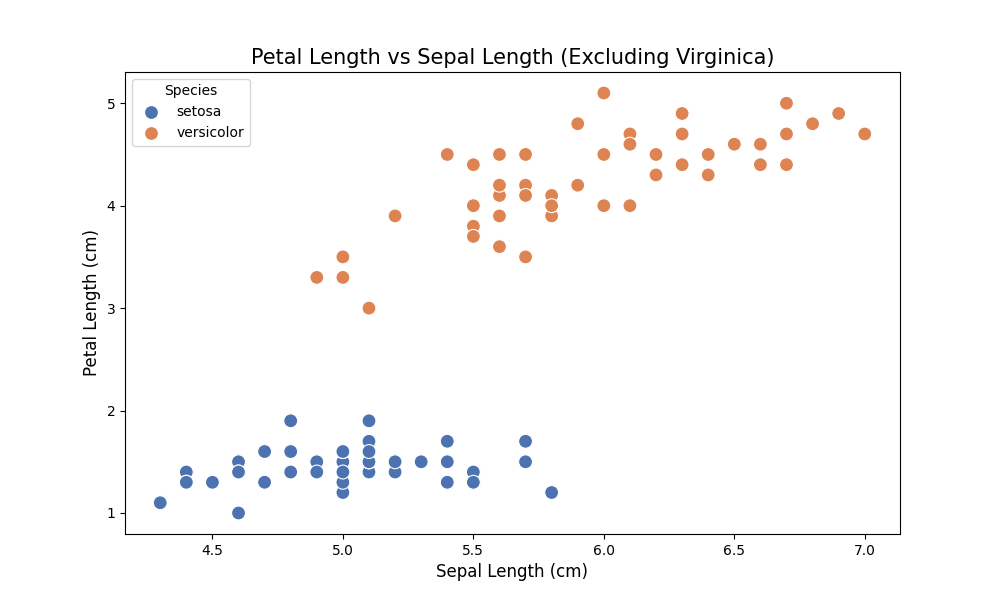
\includegraphics[scale=0.5]{figures/iris-linear-separation.png}
  \centering
  \caption{Data plot of the Iris dataset's \textit{Sepal Width} and \textit{Sepal Length} features.}
~\label{fig:iris_linear}
\end{figure} \

In Figure~\ref{fig:iris_linear} we can observe the purpose of these
modifications. By removing the \textit{virginica} class we can
linearly separate the dataset by using two different features,
e.g.\ the \textit{petal length} and \textit{sepal length}. Furthermore,
removing the feature \textit{petal width} makes the model focus on
the other features, eliminating overhead and ensuring the \ac{qml}
will converge to an optimal solution quicker. \

\subsection{Pima Indians Diabetes Dataset}\label{subsection:diabetes} \

The \ac{pid} Dataset~\cite{smith_using_1988} contains
768 data points collecting 8 features that were considered risk
factors for the onset of diabetes. This dataset presents a class
imbalance. To remediate the asymmetry in the classes distribution
we removed 232 data points from the \textit{negative} class. The
removal was performed randomly with a fixed seed to always
keep the same data points and make the results reproducible. \

A class imbalance can lead to reduced performance of a \ac{ml} model
~\cite{drummond_c45_nodate}. This decrease in accuracy could
probably be translated to \ac{qml} models as well. Therefore,
with the removal of the data points from the majority class, we
obtain a completely balanced dataset and model performance should
be maximized. \

\subsection{Wisconsin Breast Cancer (Diagnostic) Dataset} \

The Wisconsin Breast Cancer Dataset~\cite{street_nuclear_1993} is
composed by 699 data points collecting 10 features of breast masses
that could potentially be carcinogenic. While this set is also
unbalanced as the original \ac{pid} Dataset~\ref{subsection:diabetes},
the asymmetry is not as pronounced. We left the class distribution
untouched to check whether the \ac{qml} models would overcome class
distribution imbalance. \

It is interesting to note that in~\cite{winderl_quantum_2023}
they reported that normalizing the dataset per feature with the
standard deviation hindered the convergence of the \ac{qml} models.
However, we didn't experience this when training our \ac{qml} models,
thus, we do normalize the data per the feature. \

\subsection{Plus-Minus Dataset} \

~\cite{wendlinger_comparative_2024}

\subsection{MNIST Dataset} \

The MNIST Dataset~\cite{bottou_comparison_1994} is composed by
70,000 images representing handwritten individual digits between
the range from \(0\) to \(9\). Each image is a monocromatic gray scale
image shaped by \(28 \times 28 = 746\) pixels. A \ac{qml} model would
require 10 qubits to encode the features with the amplitude embedding
technique. Because the amount of operations required for the
\ac{qml} model to process the data increments exponentially, the model
quickly becomes intractable to train in commonly available hardware.
Therefore, we downsample the images by half to \(16 \times 16 = 256\) and
the \ac{qml} model would now only require 8 qubits. In Figure
~\ref{fig:mnist_resized} we can observe that downsampling the images
does not significatively visually affect the image recognition. \

\begin{figure}
  \begin{subfigure}{0.49\textwidth}
    \centering
    
\includegraphics[width = \textwidth]{figures/reshaped.jpg}
    \caption{Original image.}
  \end{subfigure}
  \begin{subfigure}{0.49\textwidth}
    \centering
    
\includegraphics[width = \textwidth]{figures/resized.jpg}
    \caption{Downsampled image.}
  \end{subfigure}
  \caption{Visual comparison between both images.}\label{fig:mnist_resized}
\end{figure} \

Similar to~\cite{winderl_quantum_2023} we further divide the MNIST
set to simulate a binary classifier and a 4-class classifier task. The
resulting datasets are named MNIST2 and MNIST4 respectively. To obtain
the MNIST2 dataset, we exclude all classes but the images that contain
a one or a nine. Furthermore, to retrieve the MNIST4 dataset we kept
all the images with digits one, three, seven and nine. With this extension
we can now compare how the \ac{qml} models accuracy varies with the
amount of classes to categorize. \

\section{State Preparation with Coherent Noise}\label{section:state_preparation_noise} \

In the next chapter (Sec.~\ref{section:vqc_training}) the trained variational circuit classifiers
utilize the amplitude embedding technique to encode classical data
into the \ac{qml} model. Pennylanes's \colorbox{inline_gray}{\lstinline|AmplitudeEmbedding|}
is utilized to encode the data accordingly. In this subsection we will
present the impact of state preparation with coherent noise on quantum
circuits. \

In order to simulate coherent noise we used Qiskit's Aer noise simulator.
Qiskit's noise models can be linked with Pennylane by declaring them as
an argument when creating a device. We attach coherent noise per gate
with the noise's corresponding unitary matrix. The unitary matrices are
derived with their respective rotational matrices \(R_{Y}\), \(R_{Z}\) and 
\(CR_{X}\) with a small \(\theta = \epsilon\). In this case we set 
\(\epsilon\) to be around 0.175 to simulate a \(10^{\circ}\) gate
miscalibration. \

The test circuits are composed first by an
\colorbox{inline_gray}{\lstinline|AmplitudeEmbedding|} state preparation
layer. Then, a single quantum gate follows that will characterize the
test circuit. In total there are three test circuits that describe the
effect of coherent noise on the \(R_{Y}\), \(R_{Z}\) and \ac{cnot} gates.
These gates were chosen because they are utilized by the strongly
entangling layers ansatz. For the rotational gates, a \(\theta = \pi\)
angle was chosen to simulate their equivalent non-rotational gates.\

In Table~\ref{tab:ry_ideal} we can observe the ideal noiseless results
for the \(R_{Y}(\pi)\) gate. This table yields the same result as applying
the Pauli Y gate. We use the Pauli Z matrix as the observable. The 
projective measurement values will be between the range of -1 and 1.

\begin{table}[h]
  \centering
  \begin{tabular}{|c|c|c|}
    \hline
    Quantum State & \(R_{Y}\left(\pi\right)\) & \(\expval{Z}\) \\
    \hline
    \(\ket{0}\) & \(i\ket{1}\) & -1 \\
    \hline
    \(\ket{1}\) & \(-i\ket{0}\) & 1 \\
    \hline
    \(\ket{+}\) & \(-i\ket{-}\) & 0 \\
    \hline
  \end{tabular}
  \caption{Expectation value with Pauli Z observable of \(R_{Y}\) gate with \(\theta = \pi\).}\label{tab:ry_ideal}
\end{table} \

The calculated expectation values for the \(R_{Y}(\theta + \epsilon)\) gate
can be found in Table~\ref{tab:ry_iso_noise}. We can observe that the
measurements from the resulting quantum state are perturbed. For the
computational basis states the expected value is equally reduced in magnitude.
For the superposition state \(\ket{+}\), the expected value 0 is shifted
by the coherent noise. The magnitude of the disturbances from the
measurements is directly proportional to \(\epsilon\). \

\begin{table}[h]
  \centering
  \begin{tabular}{|c|c|}
    \hline
    Quantum State & \(\expval{Z}\) for \(R_{Y}\left(\pi+\epsilon\right)\) \\
    \hline
    \(\ket{0}\) & -0.985 \\
    \hline
    \(\ket{1}\) & 0.985 \\
    \hline
    \(\ket{+}\) &  0.174 \\
    \hline
  \end{tabular}
  \caption{Expectation value with Pauli Z observable of \(R_{Y}\) gate with \(\theta = \pi\) and \(\epsilon = 10^{\circ}\).}\label{tab:ry_iso_noise}
\end{table} \

The experimental results from adding coherent noise to the
\(R_{Y}(\theta)\) gate are presented in Table~\ref{tab:ry_real_noise}. 
While for the \(\ket{0}\) state the result does match the calculated
-0.985 value, for the other two tested quantum states there is a
notable difference between the calculated and the experimental results. \

\begin{table}[h]
  \centering
  \begin{tabular}{|c|c|}
    \hline
    Quantum State & \(\expval{Z}\) for \(R_{Y}\left(\pi+\epsilon\right)\) \\
    \hline
    \(\ket{0}\) & -0.985 \\
    \hline
    \(\ket{1}\) & 0.940 \\
    \hline
    \(\ket{+}\) &  0.340 \\
    \hline
  \end{tabular}
  \caption{Obtained expectation value with Pauli Z observable of \(R_{Y}\) gate with \(\theta = \pi\) and \(\epsilon = 10^{\circ}\).}\label{tab:ry_real_noise}
\end{table} \

In relation to the test from the \(R_{Z}(\theta + \epsilon)\) gate, we
are not able to observe any effect of either the rotation or the noise.
This is because any Z transformation only modifies the phase of the
quantum state, which cannot be measured with the Pauli Z observable.
However, it is important to note that in the experimental results
a difference of around 0.001 was observed in the result of the \(\ket{+}\)
state measurement. \

For the \ac{cnot} gate circuit we tested both cases (a control qubit on the
first wire and a target qubit on the second wire and vice versa). For
the first case of the \ac{cnot}  gate circuit test, the noiseless expectation
values with the Pauli Z observable can be found in Table
~\ref{tab:cnot_ideal}. Similarly to the \(R_{Y}(\theta)\) circuit test,
the expectation values lie between a range of -1 and 1. Contrarily,
for the case of the \ac{cnot}  gate we measure at the end of the circuit the
two qubits from the quantum state. \

\begin{table}[h]
  \centering
  \begin{tabular}{|c|c|c|}
    \hline
    Quantum State & \ac{cnot} & \(\expval{Z}\) \\
    \hline
    \(\ket{00}\) & \(\ket{00}\) & [1, 1] \\
    \hline
    \(\ket{01}\) & \(\ket{01}\) & [1, -1] \\
    \hline
    \(\ket{10}\) & \(\ket{11}\) & [-1, -1] \\
    \hline
    \(\ket{11}\) & \(\ket{10}\) & [-1, 1] \\
    \hline
  \end{tabular}
  \caption{Expectation value with Pauli Z observable of \ac{cnot} gate.}\label{tab:cnot_ideal}
\end{table} \

In Table~\ref{tab:cnot_iso_noise} we can find the calculated
projective measurements with the Pauli Z matrix for the \ac{cnot} gate.
First of all we can observe that for the quantum states \(\ket{00}\)
and \(\ket{01}\) the values don't incur in any noise as the control
qubit is set to 0 and the Pauli X rotation is not performed on the target
qubit. Notwithstanding, for \(\ket{10}\) and \(\ket{11}\), where the
control qubit is set, noise should be present in the second qubit's
measurements with an equal magnitude. \

\begin{table}[h]
  \centering
  \begin{tabular}{|c|c|c|}
    \hline
    Quantum State & \(\expval{Z}\) \\
    \hline
    \(\ket{00}\) & [1, 1] \\
    \hline
    \(\ket{01}\) & [1, -1] \\
    \hline
    \(\ket{10}\) & [-1, -0.985] \\
    \hline
    \(\ket{11}\) & [-1, 0.985] \\
    \hline
  \end{tabular}
  \caption{Expectation value with Pauli Z observable of \ac{cnot} gate with \(\epsilon = 10^{\circ}\).}\label{tab:cnot_iso_noise}
\end{table} \

The experimental results from adding coherent noise to the
\ac{cnot} gate are presented in Table~\ref{tab:cnot_real_noise}.
Although the result for the \(\ket{00}\) state is the same as the
previously calculated value, the experimental values obtained for
the other three states differ. For the \(\ket{01}\) state there
should be no noise present, however, both qubit measurements
show disturbances in their value. Regarding the \(\ket{10}\) state
the measurement values for both qubits are inverted. Finally,
for the \(\ket{11}\) state the first qubit shows signs of noise
when it should not, while the second qubit exhibits a different noise
magnitude than calculated. \

\begin{table}[h]
  \centering
  \begin{tabular}{|c|c|c|}
    \hline
    Quantum State & \(\expval{Z}\) \\
    \hline
    \(\ket{00}\) & [1, 1] \\
    \hline
    \(\ket{01}\) & [0.992, -0.996] \\
    \hline
    \(\ket{10}\) & [-0.985, -1] \\
    \hline
    \(\ket{11}\) & [-0.992, 0.996] \\
    \hline
  \end{tabular}
  \caption{Obtained expectation value with Pauli Z observable of \ac{cnot} gate with \(\epsilon = 10^{\circ}\).}\label{tab:cnot_real_noise}
\end{table} \

In theory the effects of coherent noise should be deterministic,
as their effects can be described by a unitary matrix applied
every time once a gate has been executed. In spite of that,
the observed results from the experimental tests indicate that
coherent noise with Qiskit's noise models plugged into Pennylane
are not deterministic and fluctuate between a small margin range. \

All the gates that we tested presented differences with the
calculated and obtained results. After further investigation
we determined that the additional noise arises from the state
preparation routine. In Pennylane's documentation we found that
the \colorbox{inline_gray}{\lstinline|AmplitudeEmbedding|} function
inherits from the \colorbox{inline_gray}{\lstinline|StatePrep|}
function. Furthermore, there is a note that indicates
if \colorbox{inline_gray}{\lstinline|StatePrep|} is not supported
by the device, the method developped by Möttönen et al.~\cite{mottonen_transformation_2004}
will be utilized. \

The state preparation method proposed by Möttönen et al.\ utilizes a
combination of \(R_{Y}(\theta)\), \(R_{Z}(\theta)\) and \ac{cnot}
gates to transform a quantum state \(\ket{a}\) into another quantum state
\(\ket{b}\). For \(n\) qubits this method has an upper bound of
\(2^{n+2}-4n-4\) \ac{cnot} gates and \(2^{n+2}-5\) one-qubit elementary
rotation gates (both \(R_{Y}(\theta)\) and \(R_{Z}(\theta)\)). These
bounds grow exponentially, therefore their impact in conjunction with
quantum noise will be greatly augmented with the number of qubits used.
On the other hand, the bounds can be halved for special cases, e.g.\ when
the initial or the final quantum state is a basis vector. \

We performed some tests to see the impact state preparation has on
a quantum circuit running on Qiskit's Aer noise simulator. The experiment
consists on transforming the initial quantum state \(\ket{0_{n}}\)
(where \(n\) is the number of qubits) to the quantum state where the
magnitude of all the possible amplitude probabilities is equal. \

\begin{figure}[h!]
  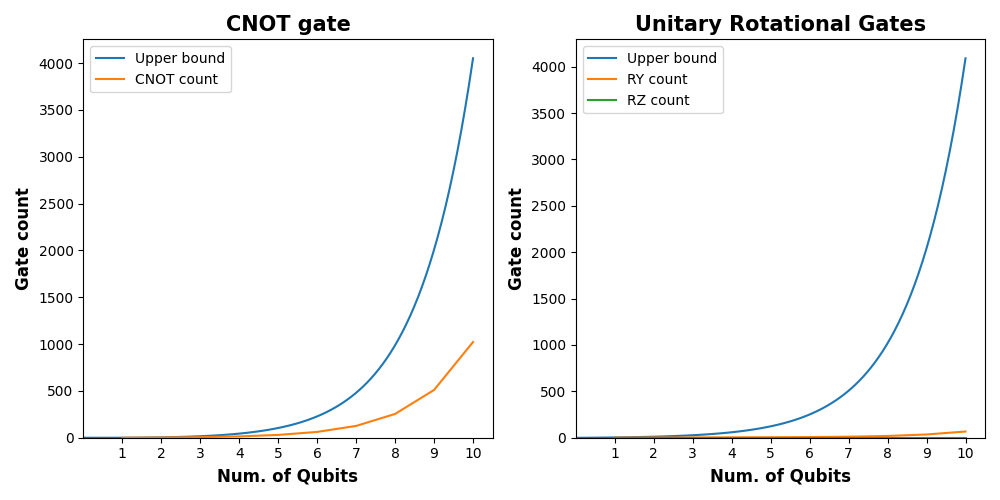
\includegraphics[scale=0.55]{figures/state-prep-gates-count.png}
  \centering
  \caption{Observed required gates to perform state preparation with Möttönen's method.}
~\label{fig:state_prep}
\end{figure} \

In Figure~\ref{fig:state_prep} the theoretical upper bounds of
Möttönen's state preparation method for both types of gates can
be distinguished from the obtained gate counts in the experiment.
While we can experimentally appreciate that the actual gate count
does not grow as fast as the theoretical upper bounds (mainly because
of the special case where we start from a computational basis vector),
we can still observe an exponential growth in the \ac{cnot} gate count.
Thus, if we perform state preparation with Möttönen's method, it will
represent a significant source of noise impacting the \ac{qml} model. \

To better comprehend the previously obtained coherent noise experimental
results we created an artificial coherent noise simulation. This
simulation utilizes Pennylane's \colorbox{inline_gray}{\lstinline|default.qubit|}
device, which does not incur in any type of noise. To artificially
introduce coherent noise into the quantum circuit we extract the
performed quantum gates Möttönen's method would use for state
preparation and after each gate introduce a corresponding rotational
gate with \(theta = \epsilon\). \

The results of the artificial coherent noise \ac{cnot} gate test are found
in Table~\ref{tab:cnot_artificial_noise}. Although they still don't
match the calculated ideal measurements from Table~\ref{tab:cnot_ideal},
we can attribute the differences to noise incurred during state preparation
using Möttönen's method. There should be no noise in any first qubit
measurement, however, for the quantum states \(\ket{10}\) and \(\ket{11}\)
state preparation for the first qubit causes noise in the measurements.
Regarding the second qubit measurements, \(\ket{10}\) and \(\ket{11}\)
should show less signs of noise. For \(\ket{01}\), there should not be
any incurred noise. Again, the differences can be attributed to noise
sustained during noise preparation. \

\begin{table}[h]
  \centering
  \begin{tabular}{|c|c|c|}
    \hline
    Quantum State & \(\expval{Z}\) \\
    \hline
    \(\ket{00}\) & [1, 1] \\
    \hline
    \(\ket{01}\) & [1, -0.940] \\
    \hline
    \(\ket{10}\) & [-0.985, -0.852] \\
    \hline
    \(\ket{11}\) & [-0.985, 0.929] \\
    \hline
  \end{tabular}
  \caption{Obtained artificial expectation value with Pauli Z observable of \ac{cnot} gate with \(\epsilon = 10^{\circ}\).}\label{tab:cnot_artificial_noise}
\end{table} \

We can look into a specific case to further specify the influence
of coherent noise during state preparation. In Equation
~\ref{eq:cnot_artificial} the quantum circuit describing the state
preparation using Möttönen's method and then applying one \ac{cnot} gate
is illustrated. The state preparation part from the quantum circuit is
enclosed by a dotted line box. The initial quantum state is \(\ket{00}\)
and it is being transformed into \(\ket{01}\) by utilizing two
\(R_{Y}(\theta)\) and two \ac*{cnot} gates. We can observe that after
each operation there is a rotational gate that correspond to the coherent
noise. \

\begin{equation}\label{eq:cnot_artificial}
  \Qcircuit @C=0.4em @R=0.4em {
    & \qw                         & \qw                    & \ctrl{1} & \ctrl{1}               & \qw                         & \qw                    & \ctrl{1} & \ctrl{1}               & \ctrl{1} & \ctrl{1}               & \meterB{Z} \\
    & \gate{R_{Y}(\frac{\pi}{4})} & \gate{R_{Y}(\epsilon)} & \targ    & \gate{R_{X}(\epsilon)} & \gate{R_{Y}(\frac{\pi}{4})} & \gate{R_{Y}(\epsilon)} & \targ    & \gate{R_{X}(\epsilon)} & \targ    & \gate{R_{X}(\epsilon)} & \meterB{Z}
    \gategroup{1}{1}{2}{9}{0.8em}{--}
  }
\end{equation} \

In this specific case, because the control qubit is set to 0, none
of the control gates will perform any modification to the target wire.
The control gates also don't modify the control qubit, thus, there are
no perturbations in the measurement. Furthermore, we can simplify
all the \(R_{Y}(\theta)\) gates into one by adding up their angles. The
resulting gate is then \(R_{Y}(\frac{\pi}{2}+2\epsilon)\). If we 
then apply the gate, we obtain the quantum state \(\ket{\psi} =
R_{Y}(\frac{\pi}{2}+2\epsilon)\ket{0}\). We can now calculate
the expectation value \(\expval{Z}{\psi}\) and the result will
be -0.940 for an \(\epsilon = 0.175\), which is exactly what we get
as a result in Table~\ref{tab:cnot_artificial_noise}. \

One important conclusion regarding this experiment is that the
quantum state \(\ket{0}\) does not require to be modified during
the state preparation routine, consequently, it will not display
any coherent noise disturbance. In addition, any control gate will
not introduce any coherent noise to the target qubit if the control
qubit is set to 0. \

Finally, in the artifical test we get deterministic measurements that
better represent coherent noise. Hence, for any further experiment
utilizing coherent noise, we will combine Pennylane's
\colorbox{inline_gray}{\lstinline|default.qubit|} with corresponding
rotational gates after each quantum gate to achieve a model closer
to reality. \

% TODO: Think why we should train AML classically and not quantum
% TODO: Think about using which type of AML
\chapter{Implementation}\label{chapter:implementation} \

In Chapter~\ref{chapter:implementation} we will introduce
the methods used to implement the experiments to answer
the research goals. In Section~\ref{section:vqa_training}
we will present how the \ac{qml} models are trained.
Futhermore, in Section~\ref{section:vqa_attacks} the
attack methodology on the \ac{vqa} model will be described. \

\section{Variational Quantum Algorithm Model Training}\label{section:vqa_training} \

In this section we will specify how the \ac{vqa} models
were trained. In Subsection~\ref{subsection:preprocess},
we will describe the dataset preprocessing methodology required
for the training. Later on in Subsection~\ref{subsection:config},
the configuration files utilized by the training pipeline will
be defined. Afterwards, in Subsection~\ref{subsection:noise_injection}
we will present how the noise is injected to the
\ac{qml} models during training and evaluation.
Finally, the developed pipeline for the training will
be presented in Subsection~\ref{subsection:pipeline}. \

\subsection{Datasets Preprocessing}\label{subsection:preprocess} \

In order to reduce the execution time of the model training, all the
datasets mentioned in the Section~\ref{section:datasets} were
stored preprocessed. All the datasets but the Plus-Minus dataset
were retrieved using OpenML~\cite{vanschoren_openml_2014}. We
obtained the Plus-Minus dataset by asking for it to the authors of 
~\cite{wendlinger_comparative_2024}. \

The preprocessing methodology encompasses for all the datasets the
removal of data points that are missing at least one feature.
Then, duplicate data points are removed to avoid overemphasizing
these elements and creating a bias in the data distribution. In
case the target labels are non-numeric, we modified them to
represent numerical classes. Finally, all the datasets except
the Iris Flower dataset are normalized using the standard
deviation and rescaled between a range of \(0\) and \(1\). This
is done with Scikit-learn~\cite{pedregosa_scikit-learn_2011}
and its purpose is to prevent feature dominance and to quicken
training convergence. \

There are two last details with regards to the preprocessing
of the datasets. Firstly, as mentioned in Subsection
~\ref{subsection:mnist}, the images from MNIST were downsampled
to be able to process them with a \ac{vqa}. Secondly, the majority
class from the \ac{pid} dataset was reduced to obtain a balanced
dataset with regards to the class distribution. \

\subsection{Configuration File}\label{subsection:config} \

The configuration files are essential to the training
pipeline. Its contents define the dataset to be used,
which type of \ac{qml} model is going to be trained,
which noise model will be injected, and some hyperparameters
regarding the \ac{qml} model's architecture. These hyperparameters
are the number of qubits, the number of layers, the number of
classes, the learning rate, the batch size, and the epochs. \

\begin{lstlisting}[language=Python, caption={Example configuration file.}, label=lst:config_file]
  {
    "dataset" : "diabetes",
    "qml_model" : "pqc",
    "noise_model" : "none",
    "num_qubits" : 3,
    "num_layers" : 40,
    "num_classes" : 2,
    "learning_rate" : 0.0005,
    "batch_size" : 16,
    "epochs" : 10
  }
\end{lstlisting}

An example configuration file can be seen in Listing
~\ref{lst:config_file}. This configuration file is given
to the training pipeline. Once the training is finished,
two more fields will be added to the configuration file.
These fields are the model accuracy on the test set and an
\(id\) to help identify the resulting model weights. The
configuration files are helpful to automate the training
and prepare the adversarial attacks on all the trained
\ac{qml} models. \

\subsection{Noise Injection}\label{subsection:noise_injection} \

The Circuit-Centric ansatz is built upon a combination of 
Pennylane's arbitrary rotation gate \colorbox{inline_gray}{\lstinline|Rot|}
and \colorbox{inline_gray}{\lstinline|CNOT|} gates. In the case
of Pennylane, the \(Rot\) gate is native to the framework, therefore,
there is no need to decompose it into other supported gates.
Nevertheless, if other frameworks or devices are utilized,
the gate decomposition is required and it would modify the resulting
trained model. \

\begin{equation}\label{eq:rot_decomposition}
  \Qcircuit @C=0.4em @R=0.4em {
    & \gate{Rot(\theta_{1},\theta_{2},\theta_{3})} & \gate{N(\epsilon)} & \qw \\
    & \gate{Rot(\theta_{1},\theta_{2},\theta_{3})} & \gate{N(\epsilon)} & \qw
  } \qquad
  \Qcircuit @C=0.4em @R=0.4em {
    & \gate{RZ(\theta_{1})} & \gate{N(\epsilon)} & \gate{RY(\theta_{2})} & \gate{N(\epsilon)} & \gate{RZ(\theta_{3})} & \gate{N(\epsilon)} & \qw \\
    & \gate{RZ(\theta_{1})} & \gate{N(\epsilon)} & \gate{RY(\theta_{2})} & \gate{N(\epsilon)} & \gate{RZ(\theta_{3})} & \gate{N(\epsilon)} & \qw
  }
\end{equation} \

Pennylane's \(Rot(\theta_{1},\theta_{2},\theta_{3})\) gate can be
decomposed in three rotational gates, namely the sequence of
\(R_{Z}(\theta_{1})\), \(R_{Y}(\theta_{2})\), and \(R_{Z}(\theta_{3})\).
If we injected the noise after every gate, the influence of noise on
the quantum circuit would increase almost three times (Eq.
~\ref{eq:rot_decomposition}). Consequently, we manually decompose the
\(Rot\) gate into its three corresponding gates to generate a single
layer in the Circuit-Centric ansatz. This will not only allow for the
pipeline in the future to be expanded and tested with new devices
and frameworks, but also will make the resuls of the thesis valid
for all of the devices and frameworks. \

In Equation~\ref{eq:rot_decomposition} the gate with the letter \(N\)
simulates the injected noise to the circuit. The type of noise model
to be injected to the \ac{qml} model is provided in the previously
described configuration file. The configuration file must then provide
one of the 6 possible noise models and either the corresponding probability
of noise to occur or the angle miscalibration \(\epsilon\). \

In order to inject noise to a \ac{qml} model we utilize Pennylane's
\colorbox{inline_gray}{\lstinline|transform|} module. We utilize it
in two different ways to create \ac{qml} models either with coherent
or incoherent noise. To simulate coherent noise we create a Pennylane
noise model object that will later on be applied to the quantum circuit.
The noise model is conformed by the addition of \(R_{Y}(\epsilon)\),
\(R_{Z}(\epsilon)\), or \(CRX(\epsilon)\) gates to the noiseless
\(R_{Y}(\theta)\), \(R_{Z}(\theta)\), or \(CNOT\) gates respectively
(where \(\epsilon\) represents the miscalibration angle). On the other
hand, to simulate incoherent noise we insert the noisy operation
depending on its type directly to the quantum circuit's gates.
This means that after every quantum gate noise might occur with
a given probability \(\epsilon\). \

For the incoherent noise \ac{qml} models, the chosen values for the
probability of noise occurring are \(2\%\), \(4\%\), \(6\%\), \(8\%\),
and \(10\%\). These values were chosen to be enough to notice an
influence in the training but not to overwhelm the classifier and
drown down any potential learning from the data. The same reasons
apply to the chosen values for the miscalibration angle for coherent
noise, the values are \(2^{\circ}\), \(4^{\circ}\), \(6^{\circ}\),
\(8^{\circ}\), and \(10^{\circ}\). \

\subsection{Training Pipeline}\label{subsection:pipeline} \

The stepping stones for the training pipeline were presented
in the previous subsections. The pipeline has been created
in order to simplify and automatize the training of the
\ac{qml} models. The pipeline is based on the configuration
files. Each \ac{qml} model requires a configuration file to
be trained, therefore, the amount of configuration files
depends on the number of models to be trained. \

In this thesis we are training \ac{qml} models for \(7\)
datasets, with \(6\) noise types with each one having \(5\)
different miscalibrations or probabilities. Adding up
the \(7\) noiseless models, we end up with \(217\) configuration
files and \ac{qml} models to be trained. Manually creating
the configuration files would take a considerable
amount of time. Therefore, we coded a script to
automatically create the configuration files of a
given dataset. \
% 7 * 6 * 5 = 210 + 7 (noiseless) = 217

After the configuration files have been created,
we can start with the training. Training \(217\)
\ac{qml} models individually is also time consuming.
Thus, we created a script that retrieves all
the configuration files from a specific dataset
and performs the model training. More importantly,
the resulting weights of the model are automatically
saved in conjunction with the modified configuration
files. This serves two purposes. Firstly, we need the model
weights to evaluate their accuracy when performing the
adversarial attacks. Secondly, the pipeline checks
if the model has already been previously trained and
can skip retraining it. Therefore, the automated training
can be interrupted and resumed without losing any information
about the trained models. \

The actual model training is performed by using a training loop
based on the PyTorch Lightning~\cite{falcon_pytorch_2019} workflow.
To enable the Lightning workflow we created a helper file with
utility functions that help train and evaluate the \ac{qml} model.
In this file we define the training, validation and testing steps.
Additionally, we implement helper functions to calculate the 
accuracy and a threshold method to be able to evaluate the \ac{qml}
model. Finally, we define the model architecture based on the
weights, number of target labels to classify and a forward pass. \

The Lightning workflow simplifies and streamlines the training.
Nevertheless, in order to perform the training loop, a small
setup before is required. First of all, based on the configuration
file we retrieve the datasets. If the dataset has already been
fetched, we simply load the preprocessed dataset from the local files.
Later on, we define the \ac{qml} model based on the given hyperparameters.
Moreover, the required weights for training the module are randomly
initialized. \

% TODO: Mention specific hyperparameters / qml model architectures per dataset in a table

Once the preprocessed dataset has been loaded, we divide it into
different sets to facilitate the training loop. For most of
the datasets we have a \(70/30\) split between the training
set and the test set. The test set is stratified according
to the data distribution from the training set. For the
MNIST and Plus-Minus datasets only \(20\%\) of the dataset
is used for training, as theses datasets are substantially
more computationally demanding than the other datasets. Moreover,
for the MNIST datasets we have a \(70/15/15\) training, 
validation, and test set split respectively. \

The last requirements for the training loop to be prepared are the
loss functionand the optimizer used to the adapt the \ac{qml} model. In our
specific case we utilize ADAM, a gradient-based optimizer, as it will
lead to faster convergence than just using a gradient descent. For the
loss function we utilize PyTorch's implementation of the Cross Entropy
Loss, therefore, we interpret the resulting measurements from the
\ac{qml} model similar to a probability distribution.  \

Once everything is set up, we let the \textit{Trainer} module
perform the training of the \ac{qml} model. The \textit{Trainer}
module is responsible for loading the data points in the given
batch number, calculating the loss, and optimizing the \ac{qml}
models weights towards convergence. We also implemented an early
stopping mechanism when the training accuracy reaches \(100\%\)
to avoid overfitting the simpler models. \

With this implemented pipeline it is simple to perform
any further updates. The helping files are modularly
designed to be reused, modified, and updated. Incorporating
new and different types of \ac{qml} models with noise
injection is simple. Furthermore, the chosen noise types
and values can be effortlessly modified and expanded. 
Not only does the pipeline enable the replication of results,
but the creation of new experimentats. \

\section{Adversarial Attacks on Variational Quantum Algorithm Model}\label{section:vqa_attacks} \

In this section we will specify how the adversarial
attacks and evaluation are performed. In Subsection
~\ref{subsection:adv_attacks}, we will describe the process
to obtain adversarial examples with the \ac{fgsm} and \ac{pgd}
techniques. Afterwards in Subsection~\ref{subsection:evaluation},
the evaluation procedure of the trained \ac{qml} models against
adversarial examples will be defined. \

\subsection{Adversarial Attacks}\label{subsection:adv_attacks}\

Similar to the training pipeline introduced in the previously
section, we tried to automate and simplify as much as possible
the creation of the adversarial examples. In our thesis we
are utilizing two different adversarial techniques, namely
\ac{fgsm} (Subsec.~\ref{subsection:fgsm}) and \ac{pgd}
(Subsec.~\ref{subsection:pgd}). \

Instead of manually implementing the attacks, there are
several Python libraries that already have coded functions according
to different techniques to create adversarial examples. In our
case we utilize Cleverhans~\cite{papernot_technical_2018} due
to its easeness of use and its interface with PyTorch models.
This allows our previous PyTorch \ac{qml} model definition to
be used as an input for the attack functions. \

The function to create adversarial examples using the
\ac{fgsm} technique requires the previously mentioned
PyTorch \ac{qml} model. Additionally, it requires the
input data point to attack. We can provide as an argument
whether it is a targeted attack or not. In our specific
case we are creating untargeted adversarial examples,
therefore, we don't have to specify a target label.
Moreover, we indicate the \(L_{\infty}\) norm to be used,
as it causes small uniform distributions across all
the features that are harder to perceive. Finally,
we must determine the attack strength \(\epsilon\). \

The function that implements the \ac{pgd} method
requires all the previously mentioned arguments
for the \ac{fgsm} technique. Additionally, it
also needs the iterative step size and the
number of iterations to recurringly create the
adversarial examples. These specific arguments are
set to \(0.01\)  and \(40\) respectively. \

The noiseless \ac{qml} model is used as the required
PyTorch model for crafting the adversarial examples.
Thus, we retrieve the pretrained weights according to the
\ac{qml} model and the dataset we are targeting.
This will enable us to create a baseline attack
and check whether the noisy training improves
the resilience of the models against adversarial
attacks. \

Once the dataset has been retrieved, we perform
both attacks on the test set to create the adversarial
examples needed to evaluate the noisy \ac{qml} models.
We evaluate directly the performance of the noiseless
model with the adversarial examples to verify that
the performed attacks are correctly implemented and
that they are misclassified by the model they are
intended to fool. This process is repeated 5 times,
each with a different value for the attack strength
\(\epsilon\). The result of this process is obtaining
10 different variations of the adversarial examples with
increasing difficulty to be correctly classified. This will
allow us to quantify how resilient the noisy \ac{qml}
models are in case they are actually more robust
against adversarial attacks. \

While for image data the modifications to obtain the adversarial
examples are conceptually simple to understand (Fig.
~\ref{fig:adversarial_example}), for the tabular data it
might be more abstract to understand the changes. In Figure
~\ref{fig:adversarial_tabular} we show the effects of \ac{fgsm}
on two dimensions of a data point for the Iris dataset. We use
two dimensions only to simplify the understanding of what
disturbances are added to tabular data. \

\begin{figure}[h!]
  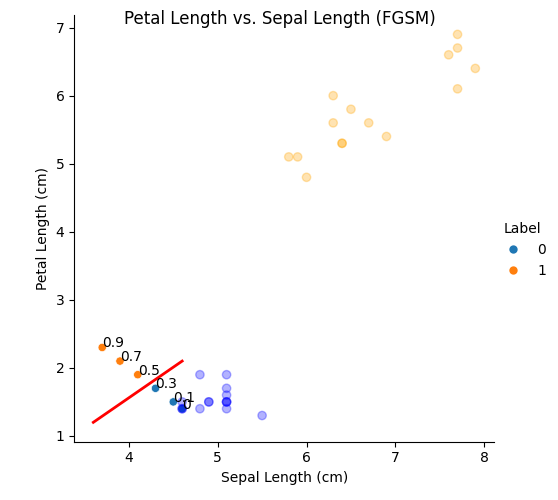
\includegraphics[scale=0.75]{figures/tabular-adversarial.png}
  \centering
  \caption{Effects of \ac{fgsm} on the Iris dataset's \textit{Petal Length} and \textit{Sepal Length} features for different attack strengths.}
~\label{fig:adversarial_tabular}
\end{figure} \

We can observe that the data point wihout any modifications
is classified with the label \(0\). With an increasing attack
strength the data point is modified such that the \textit{Sepal
Lenght} is reduced while the \textit{Petal Length} is increased.
The red line in this case represents the classification threshold,
where the \ac{qml} classifier starts labeling the data point as
\(1\) instead of \(0\). Once the features have been adapted
accordingly to exceed the classification threshold, the \ac{qml}
model will start to misclassify the data point. \

In the case of attacking a binary classificator, utilizing
a technique implementing an untargeted attack is equivalent
to executing a targeted attack aiming to obtain a misclassification
with the datapoint's contrary class. Therefore, for binary
classificators there is no distinction between performing a
targeted or an untargeted attack. However, this is not the case when
the \ac{qml} model is trying to differentiate between more than
two classes, as the result of an untargeted attack can now
be classified into more than one category. \

The attack strength regulates the magnitude of the perturbations
added to the original input to create the adversarial examples. 
In this thesis we chose \(5\) different attack strengths,
specifically the values \(\left[0.1, 0.3, 0.5, 0.7, 0.9\right]\).
This allows us to slowly increase the attack strength while
checking over a big range how the noisy and noisless \ac{qml}
models react. Another factor that influenced this range is that
the attacks are being applied to the preprocessed data points
that have been normalized and rescaled. \

\subsection{Automated Evaluation}\label{subsection:evaluation} \

Continuing the idea of the pipeline, evaluating the trained
\ac{qml} models should be simple to execute. The evaluation
requires two arguments, namely the dataset and a given \ac{qml}
model type to assess. The evaluation code will then
automatically calculate the accuracy scores of all the \(31\)
(Subsection~\ref{subsection:pipeline}) trained models. Additionally,
it also evaluates the \ac{qml} models against the two different
adversarial attacks with five differing attack strength.
The evaluation pipeline then results per dataset on \(310 + 31 = 341\)
data points to be analysed. \

In order to avoid performing a redundant assessment, first,
the pipeline will check if the evaluation and the figures
have already been created. If any of the two is missing,
the pipeline will automatically calculate the \ac{qml} models'
accuracies and draw the figures from the resulting data. To
do this, it verifies that all the adversarial samples have
already been crafted. \

The evaluation process iterates over all the noise
models (and its miscalibrations or noise probabilities)
and assesses each model with the modified adversarial
examples. The adversarial evaluation calculates first the
\ac{qml} model's accuracy against the unmodified test set.
Later on, the evaluation script retrieves the adversarial
examples for both adversarial attack techniques and their
variations and computes the adversarial accuracy of the model.
The results of this evaluation are saved in a file
for further use when creating the figures comparing the
accuracy of the different models in differents scenarios. \

The resulting file from the evaluation process stores the
accuracies and the characteristics of the models. Per dataset,
we can retrieve \(31\) clean accuracies without any attack
performed and \(310\) adversarial accuracies, this corresponds
to the previosly mentioned \(341\) cipher. This information
is required by the figure creation process. \

The graph creation process will output \(16\) different
figures belonging to \(3\) different types of graphs. Each
type of graph tries to convey a different comparison between
the different \ac{qml} models. The first type of grpah.  \

Mention the graph creation (probs reference notebook notes),
state the 3 differents types of graphs created and how to read
them. Accuracy on clean samples with noise model, Accuracy of
noiseless model being attacked, accuracy of noisy models being attacked. \
\chapter{Results}\label{chapter:results} \

In Chapter~\ref{chapter:results} we will introduce
the results of the experiments presented in Chapter
~\ref{chapter:implementation}. The results will be presented
per dataset. Each dataset contains two graphs related to
the model accuracy on the clean test set for noisy and
noiseless models. Additionally, two more graphs are
introduced to portray the effect of the adversarial
attacks on the noiseless \ac{qml} model, one for each
attack with increasing attack strengths. Finally, two
graphs for each of the six noise models are provided.
These last graphs will provide insights of the effects
of the diverse quantum noise sources with different noise 
magnitudes on the adversarial accuracy of both adversarial
attacks. \

In Section~\ref{section:iris-eval} the results from
the Iris dataset are shown. In Section~\ref{section:diabetes-eval}
the results from the \ac{pid} dataset follow. Moreover,
in Section~\ref{section:breast-cancer-eval} the outcomes
for the Wisconsin Breast Cancer dataset can be found.
Lastly, the experiments' outcomes from the Plus-Minus dataset
are provided in Section~\ref{section:plus-minus-eval}. \

\section{Iris Dataset}\label{section:iris-eval} \

The results obtained from training the noisy and noiseless
\ac{qml} models on the Iris dataset can be found in Subsection
~\ref{subsection:iris-noisy-acc}. Moreover, the outcomes
of both adversarial attacks will be presented in Subsection
~\ref{subsection:iris-adv-acc}. Finally, the evaluation
of the noisy models against the adversarial attacks can
are presented in Subsection~\ref{subsection:iris-noisy-adv-acc}. \

\subsection{Noisy Models Accuracy}\label{subsection:iris-noisy-acc} \

In Figure~\ref{fig:iris-12} we can observe the results
from the training of noiseless and noisy \ac{qml} models
for the Iris test dataset. The noiseless baseline model accuracy
can be found on both graphs at the y-intercept, which in
this case is of \(100\%\). We note in Subfigure~\ref{fig:iris1}
that for the Iris dataset there are no perceptible
repercussions on the model accuracy when training with
coherent noise and remains the same as the noiseless
baseline performance. \

Nevertheless, for incoherent noise models in Subfigure
~\ref{fig:iris2} we can already observe a decrease in
model accuracy for certain noise models. For depolarizing
noise and bit-flip induced noise we notice the same behavior
as with coherent noise, remaining constant throughout
the different noise magnitudes and obtaining the same
performance as the noiseless model. \

Regarding phase damping noise, the model performance
marginally decreases the accuracy to \(97\%\) starting at
\(8\%\) noise probability. For phase-flip induced noise
the model performance slightly decreases in comparison
to phase damping noise to \(90\%\) at \(6\%\) noise probability
until the accuracy decreases to \(86\%\) at \(10\%\). Moreover,
for amplitude damping noise we can appreciate that the model
performance oscilates significantly starting \(4\%\) noise
probability. Furthermore, amplitude damping \ac{qml}
model's accuracy is significantly lower than other noiseless
and noisy models, reaching \(50\%\) accuracy at \(10\%\)
noise probability. \

\begin{figure}[!h]
  \centering

  \begin{subfigure}{0.45\textwidth}
      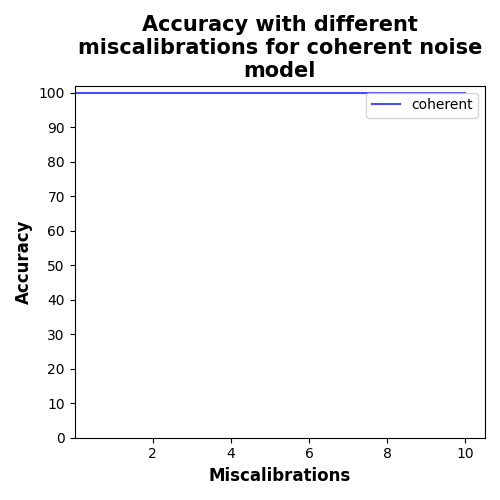
\includegraphics[width=\linewidth]{figures/evaluation_results/iris/pqc/figures/accuracy-coherent.png}
      \subcaption{Coherent noise model's accuracy.}
      \label{fig:iris1}
  \end{subfigure} \qquad
  \begin{subfigure}{0.45\textwidth}
      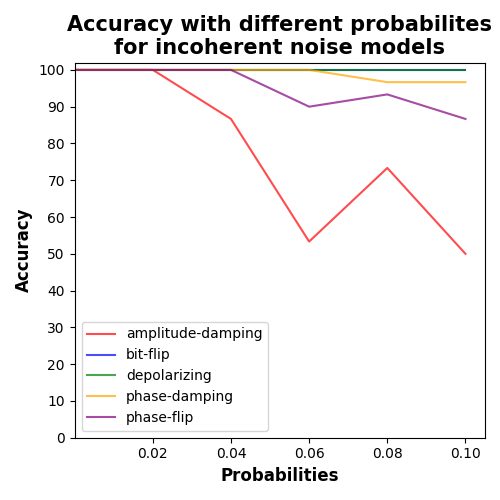
\includegraphics[width=\linewidth]{figures/evaluation_results/iris/pqc/figures/accuracy-incoherent.png}
      \subcaption{Incoherent noise models' accuracy.}
      \label{fig:iris2}
  \end{subfigure}

  \caption{\ac{vqa}'s accuracy on the Iris clean test dataset.}
  \label{fig:iris-12}
\end{figure} \

\subsection{Adversarial Accuracy}\label{subsection:iris-adv-acc} \

In Figure~\ref{fig:iris-34} we introduce the effects of the
adversarial attacks on the accuracy of the noiseless \ac{qml}
model. As expected, we can observe that for both adversarial
techniques the performance of the model decreases with increasing
attack strength. For the \ac{fgsm} technique in Subfigure~\ref{fig:iris3}
we notice a stark accuracy decrease until it stabilizes to around
\(50\%\) after \(0.5\) attack strength. Furthermore, in Subfigure
~\ref{fig:iris4} for the \ac{pgd} technique we see a lesser performance
decrease that stabilizes to around \(70\%\) after \(0.5\) attack strength. 
That \ac{fgsm} has a bigger performance impact than \ac{pgd} is expected
as \ac{fgsm}'s perturbations tend to be bigger in magnitude and more
disruptive to the input. \

\begin{figure}[!h]
  \centering

  \begin{subfigure}{0.45\textwidth}
      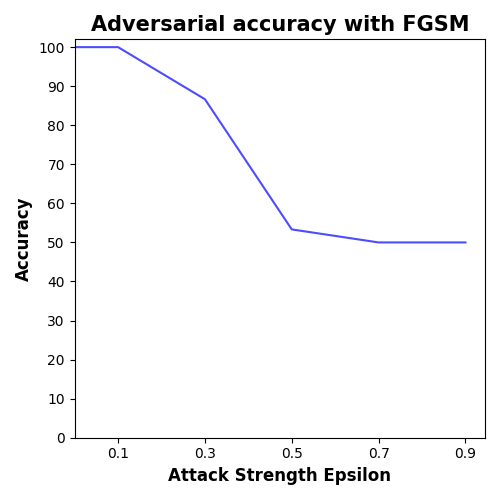
\includegraphics[width=\linewidth]{figures/evaluation_results/iris/pqc/figures/none-fgsm.png}
      \subcaption{Noiseless model's \ac{fgsm} adversarial accuracy.}
      \label{fig:iris3}
  \end{subfigure} \qquad
  \begin{subfigure}{0.45\textwidth}
      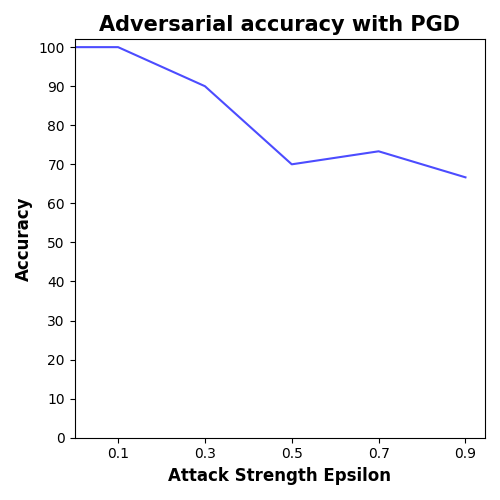
\includegraphics[width=\linewidth]{figures/evaluation_results/iris/pqc/figures/none-pgd.png}
      \subcaption{Noiseless model's \ac{pgd} adversarial accuracy.}
      \label{fig:iris4}
  \end{subfigure}

  \caption{\ac{vqa}'s accuracy on the adversarial Iris test dataset.}
  \label{fig:iris-34}
\end{figure} \

\subsection{Noisy Models Adversarial Accuracy}\label{subsection:iris-noisy-adv-acc} \

In this subsection we introduce the results from performing
the adversarial attacks on the noisy models with different noise
magnitudes for the Iris dataset. In each graph the color gray
represents the baseline adversarial accuracy obtained by the
noiseless model. \

In Figure~\ref{fig:iris-56} we present the outcomes from the amplitude
damping noisy models evaluation. For \ac{fgsm} in Subfigure~\ref{fig:iris5}
we note that the model with \(2\%\) noise probability obtains the same
performance as the noiseless model. Furthermore, we observe that an
increase in noise probability when training in general does not equate
to a worse adversarial accuracy at lower attack strengths, as the model
with \(8\%\) noise probability performs better than the one with \(6\%\)
noise probability. Nevertheless, once the attack strength reaches a
value of \(0.9\) all the models perform equally, converging to \(50\%\)
accuracy. \

\begin{figure}[!h]
  \centering

  \begin{subfigure}{0.45\textwidth}
      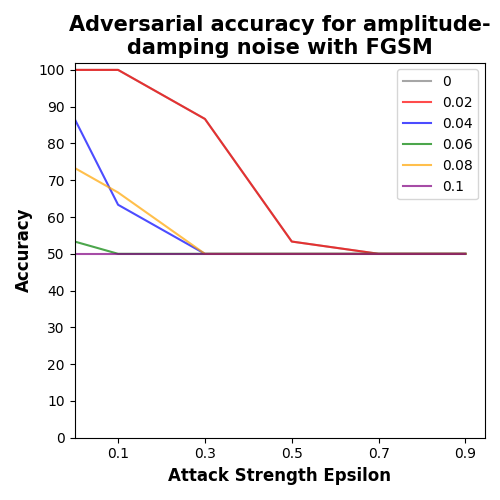
\includegraphics[width=\linewidth]{figures/evaluation_results/iris/pqc/figures/amplitude-damping-fgsm.png}
      \subcaption{Amplitude damping noise model's \ac{fgsm} adversarial accuracy.}
      \label{fig:iris5}
  \end{subfigure} \qquad
  \begin{subfigure}{0.45\textwidth}
      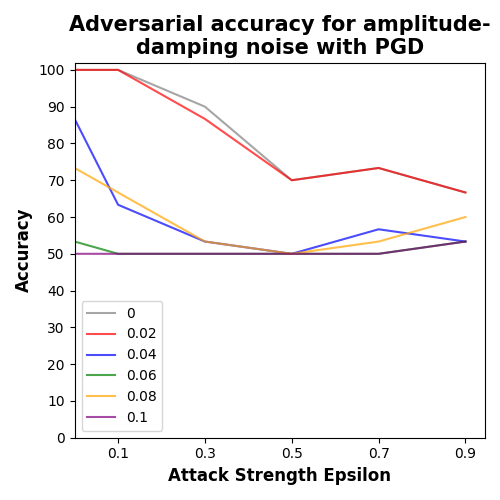
\includegraphics[width=\linewidth]{figures/evaluation_results/iris/pqc/figures/amplitude-damping-pgd.png}
      \subcaption{Amplitude damping noise model's \ac{pgd} adversarial accuracy.}
      \label{fig:iris6}
  \end{subfigure}
  \caption{Amplitude damping noise models' accuracy on the adversarial Iris test dataset.}
  \label{fig:iris-56}
\end{figure} \

In Subfigure~\ref{fig:iris6} we introduce the results from the \ac{pgd}
attack on the amplitude damping noisy models. As with the \ac{fgsm} attack
we can observe that the best performing model (close to the noiseless
model's performance) is the one with the smallest noise probability. Also,
we can note that increasing noise probability does not equal a direct
decrease in adversarial accuracy at lower attack strengths. Nevertheless,
noisy models in general perform significantly worse than the noiseless
model. Interestingly, when the attack strength surpasses \(0.5\), all
the noisy models (with the exception of the model with \(2\%\) noise
probability) perform slightly better than at lower attack strengths. \

In Figure~\ref{fig:iris-78} we present the outcomes from the bit-flip
noisy models evaluation. For \ac{fgsm} in Subfigure~\ref{fig:iris7}
we note that there are some models (\(2\%, 4\%, 10\%\)) performing
better than the noiseless model, while others (\(6\%, 8\%\)) have
a lower or equal adversarial accuracy throughout the different
attack strengths. While the model trained with \(10\%\) noise
probability performs the best against attack strength's lower
than \(0.7\), the adversarial accuracy drops to around \(33\%\)
(the lowest recorded accuracy) at an attack strength of \(0.9\). \

\begin{figure}[!h]
  \centering

  \begin{subfigure}{0.45\textwidth}
      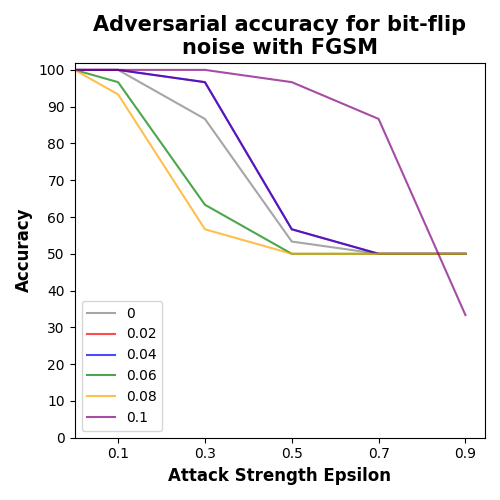
\includegraphics[width=\linewidth]{figures/evaluation_results/iris/pqc/figures/bit-flip-fgsm.png}
      \subcaption{Bit-Flip noise model's \ac{fgsm} adversarial accuracy.}
      \label{fig:iris7}
  \end{subfigure} \qquad
  \begin{subfigure}{0.45\textwidth}
      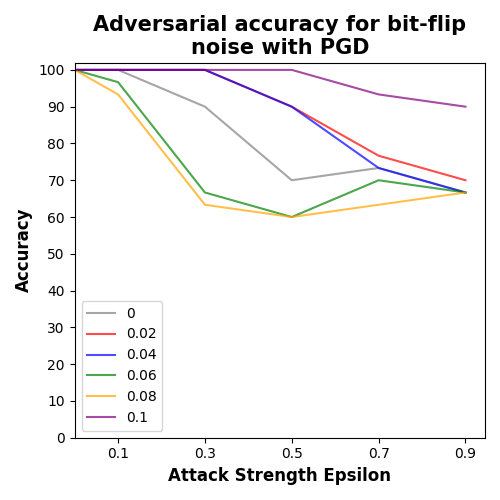
\includegraphics[width=\linewidth]{figures/evaluation_results/iris/pqc/figures/bit-flip-pgd.png}
      \subcaption{Bit-Flip noise model's \ac{pgd} adversarial accuracy.}
      \label{fig:iris8}
  \end{subfigure}
  \caption{Bit-Flip noise models' accuracy on the adversarial Iris test dataset.}
  \label{fig:iris-78}
\end{figure} \

In Subfigure~\ref{fig:iris8} we introduce the results from the \ac{pgd}
attack on the bit-flip noisy models. Similar to the \ac{fgsm} performance,
the models with noise probability (2\%, 4\%, and 10\%) perform better or equal
than the baseline noiseless adversarial accuracy. Nevertheless, the stark
performance drop from the model trained with 10\% noise probability
at 0.9 attack strength does not occur in this case. Furthermore, analogous
to the \ac{fgsm} results, the models trained with (6\% and 8\%) noise
probability perform worse than the noiseless model. However, with attack
strengths higher than 0.5, these models actually see a slight performance
increase to match the baseline model at 0.9 attack strength. \

In Figure~\ref{fig:iris-910} we present the outcomes from the coherent
noisy models evaluation. For \ac{fgsm} in Subfigure~\ref{fig:iris9}
we note that all the noisy models perform better than the noiseless
models throught almost all of the attack strength range. Only at 
attack strength 0.9 do the models with a misconfiguration of 2 and
4 degrees have a marginally lower accuracy than the noiseless model's
accuracy. In this specific case, there seems to be a slight correlation
between model robustness and degree misconfiguration, where the
higher the misconfiguration degree leads to a more robust model. The
two models with the highest coherent noise (8 and 10 degrees) achieve
an adversarial accuracy of around 96\% at the highest attack strength. \

\begin{figure}[!h]
  \centering

  \begin{subfigure}{0.45\textwidth}
      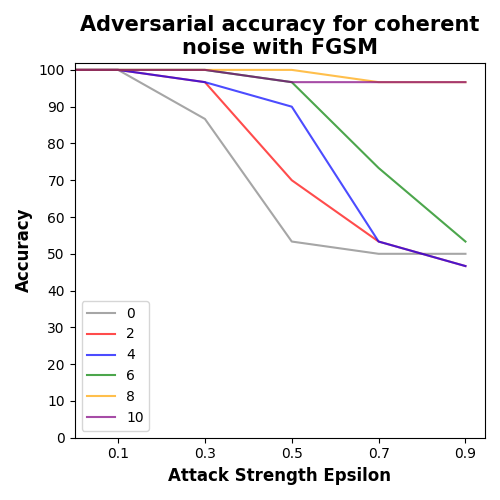
\includegraphics[width=\linewidth]{figures/evaluation_results/iris/pqc/figures/coherent-fgsm.png}
      \subcaption{Coherent noise model's \ac{fgsm} adversarial accuracy.}
      \label{fig:iris9}
  \end{subfigure} \qquad
  \begin{subfigure}{0.45\textwidth}
      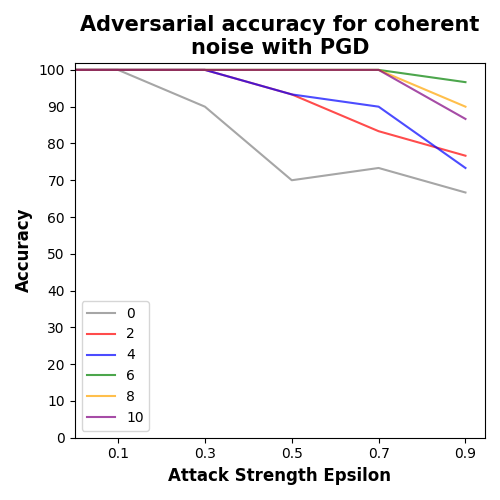
\includegraphics[width=\linewidth]{figures/evaluation_results/iris/pqc/figures/coherent-pgd.png}
      \subcaption{Coherent noise model's \ac{pgd} adversarial accuracy.}
      \label{fig:iris10}
  \end{subfigure}
  \caption{Coherent noise models' accuracy on the adversarial Iris test dataset.}
  \label{fig:iris-910}
\end{figure} \

In Subfigure~\ref{fig:iris10} we introduce the results from the \ac{pgd}
attack on the coherent noisy models. Comparable to the results from the
\ac{fgsm} evaluation, all the coherent noisy models perfom better than
the baseline noiseless model benchmark. Furthermore, the coherent noisy
models with a lower misconfiguration degree obtain a lower adversarial
accuracy than the models with a higher noise disturbance. Thus, we can
derive a slight correlation with the degree of misconfiguration and the
adversarial accuracy. \

In Figure~\ref{fig:iris-1112} we present the outcomes from the depolarizing
noisy models evaluation. For \ac{fgsm} in Subfigure~\ref{fig:iris11}
we note that all the noisy models but the one with 2\% noise probability
perform at equal or better than the noiseless benchmark until the attack
strength 0.7 is reached. The model with 4\% noise probability is the best
model in this range. However, this model's adversarial accuracy significantly
drops to the lowest value recorded at around 26\% with attack strength's
higher than 0.7. While most of the noisy models have a higher adversarial
accuracy than the noiseless model throughout the attack strength range,
no direct correlation can be drawn between the noise probability and the
model's robustness. \

\begin{figure}[!h]
  \centering

  \begin{subfigure}{0.45\textwidth}
      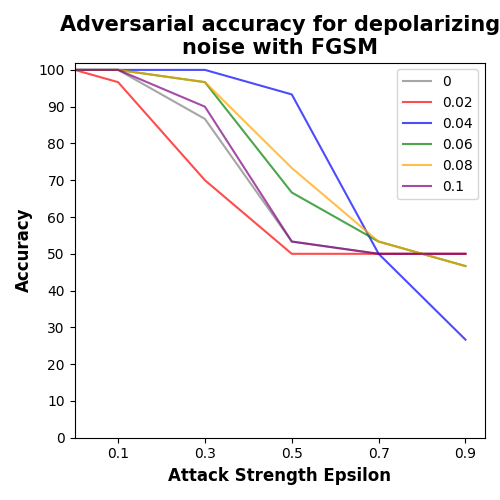
\includegraphics[width=\linewidth]{figures/evaluation_results/iris/pqc/figures/depolarizing-fgsm.png}
      \subcaption{Depolarizing noise model's \ac{fgsm} adversarial accuracy.}
      \label{fig:iris11}
  \end{subfigure} \qquad
  \begin{subfigure}{0.45\textwidth}
      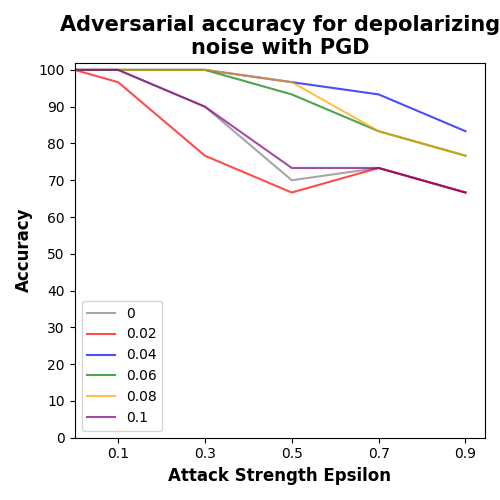
\includegraphics[width=\linewidth]{figures/evaluation_results/iris/pqc/figures/depolarizing-pgd.png}
      \subcaption{Depolarizing noise model's \ac{pgd} adversarial accuracy.}
      \label{fig:iris12}
  \end{subfigure}
  \caption{Depolarizing noise models' accuracy on the adversarial Iris test dataset.}
  \label{fig:iris-1112}
\end{figure} \

In Subfigure~\ref{fig:iris12} we introduce the results from the \ac{pgd}
attack on the depolarizing noisy models. Comparable to the results from
the \ac{fgsm} model evaluation, all models except the one with 2\% noise
probability perform equal or better than the noiseless model throughout
the whole attack strength spectrum. The 4\% noise probability model is
still the best but now doesn't suffer a big drop-off at 0.9 attack strength
like in the \ac{fgsm} outcomes. This model reaches around 83\% adversarial
accuracy with the highest tested attack strength. In this case, although
most of the noisy models have a higher accuracy than the noiseless model,
no correlation can be drawn between model robustness and noise propensity. \

In Figure~\ref{fig:iris-1314} we present the outcomes from the phase damping
noisy models evaluation. For \ac{fgsm} in Subfigure~\ref{fig:iris13}
we note that the models with intermediate noise probabilities (4\% and 6\%)
perform marginally better than the baseline noiseless model up until the
attack strength 0.7. Contrarily, the remaining noise probability models 2\%,
8\% and 10\% obtain a lower adversarial accuracy than the noiseless model.
While some noisy models perform better than the benchmark set by the noiseless
model, no relation between the noise magnitude and the model robustness can
be derived. \

\begin{figure}[!h]
  \centering

  \begin{subfigure}{0.45\textwidth}
      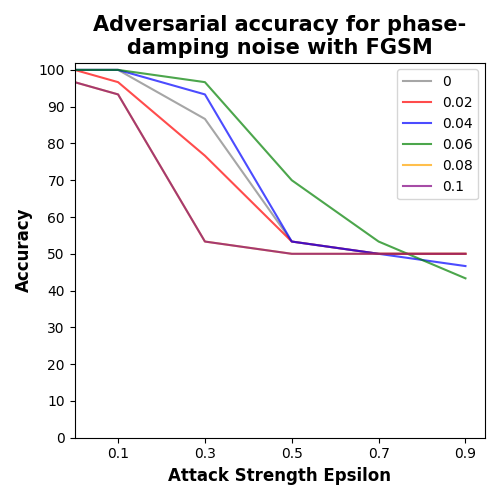
\includegraphics[width=\linewidth]{figures/evaluation_results/iris/pqc/figures/phase-damping-fgsm.png}
      \subcaption{Phase Damping noise model's \ac{fgsm} adversarial accuracy.}
      \label{fig:iris13}
  \end{subfigure} \qquad
  \begin{subfigure}{0.45\textwidth}
      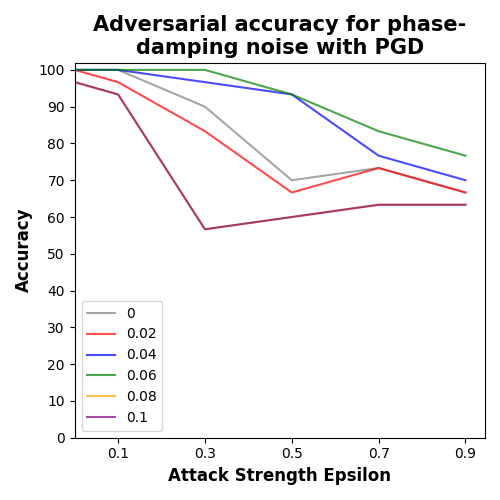
\includegraphics[width=\linewidth]{figures/evaluation_results/iris/pqc/figures/phase-damping-pgd.png}
      \subcaption{Phase Damping noise model's \ac{pgd} adversarial accuracy.}
      \label{fig:iris14}
  \end{subfigure}
  \caption{Phase damping models' accuracy on the adversarial Iris test dataset.}
  \label{fig:iris-1314}
\end{figure} \

In Subfigure~\ref{fig:iris14} we introduce the results from the \ac{pgd}
attack on the phase damping noisy models. The adversarial accuracies
obtained with the \ac{pgd} technique show the same behavior than the
values obtained by the \ac{fgsm} attack. The main difference lies
on the magnitude of the adversarial accuracies, were the results
from the \ac{pgd} tests are slightly higher than for the \ac{fgsm}
experiments. \

In Figure~\ref{fig:iris-1516} we present the outcomes from the phase-flip
noisy models evaluation. For \ac{fgsm} in Subfigure~\ref{fig:iris15}
we note that only the model with the lowest noise probability (2\%)
obtains a higher adversarial accuracy than the baseline noiseless
model. This relationship is maintained up until the 0.7 attack strength,
where the noisy model performance is marginally lower than the noiseless
model. The performance of both types of model, noisy and noiseless,
converges to around 50\% at the highest attack strength. \

\begin{figure}[!h]
  \centering

  \begin{subfigure}{0.45\textwidth}
      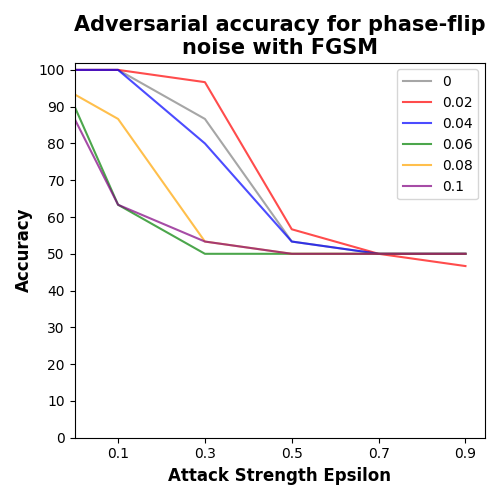
\includegraphics[width=\linewidth]{figures/evaluation_results/iris/pqc/figures/phase-flip-fgsm.png}
      \subcaption{Phase-Flip noise model's \ac{fgsm} adversarial accuracy.}
      \label{fig:iris15}
  \end{subfigure} \qquad
  \begin{subfigure}{0.45\textwidth}
      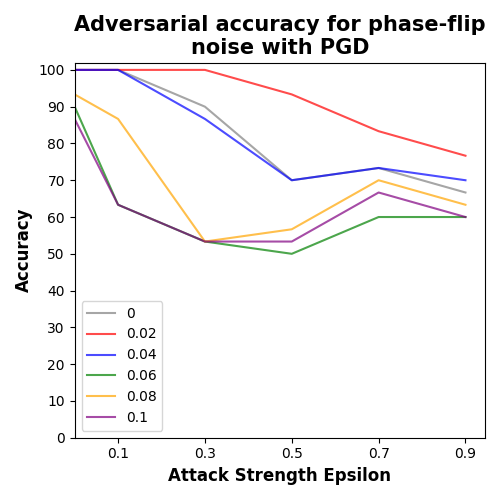
\includegraphics[width=\linewidth]{figures/evaluation_results/iris/pqc/figures/phase-flip-pgd.png}
      \subcaption{Phase-Flip noise model's \ac{pgd} adversarial accuracy.}
      \label{fig:iris16}
  \end{subfigure}

  \caption{Phase-Flip noise models' accuracy on the adversarial Iris test dataset.}
  \label{fig:iris-1516}
\end{figure} \

In Subfigure~\ref{fig:iris16} we introduce the results from the \ac{pgd}
attack on the phase-flip noisy models. Similar to the results from the
\ac{fgsm} attack, only the model with 2\% noise probability performs
better than the noiseless model. Nevertheless, in the case of the \ac{pgd}
adversarial accuracies this behavior is found throughout all the attack
strength range. The performance of the remaining noisy models unexpectedly
either slightly increases or stays the same with increasing attack strength
starting a strength calue of 0.5. For both, the \ac{pgd} and the
\ac{fgsm} attack techniques we can observe a small correlation between the
model robustness, where a higher noise probability equals lesser model
performance. The model with 6\% noise probability is the exception to
this trend because it has the lowest adversarial accuracies throughout
the whole attack strength range. \

\section{\acl{pid} Dataset}\label{section:diabetes-eval} \

The results obtained from training the noisy and noiseless
\ac{qml} models on the \ac{pid} dataset can be found in Subsection
~\ref{subsection:diabetes-noisy-acc}. Moreover, the outcomes
of both adversarial attacks will be presented in Subsection
~\ref{subsection:diabetes-adv-acc}. Finally, the evaluation
of the noisy models against the adversarial attacks can
are presented in Subsection~\ref{subsection:diabetes-noisy-adv-acc}. \

\subsection{Noisy Models Accuracy}\label{subsection:diabetes-noisy-acc} \

In Figure~\ref{fig:diabetes-12} we can observe the results
from the training of noiseless and noisy \ac{qml} models
for the \ac{pid} test dataset. The noiseless baseline model accuracy
can be found on both graphs at the y-intercept, which in
this case is of 67.7\%. We note in Subfigure~\ref{fig:diabetes1}
that for the \ac{pid} dataset the model accuracy slightly decreases
when training with an increasing coherent noise effect. The model
performance is slowly reduced until it reaches 49\% accuracy. \

For incoherent noise models in Subfigure~\ref{fig:diabetes2}
we can observe a decrease in model accuracy for all the noise
models. In this case, phase damping noise performs the best
of any noise models, followed then by models with amplitude
damping noise. They each have an accuracy of 59\% and 49\% on the clean
test dataset respectively, which represents a lower performance
than the noiseless model's accuracy. \

Regarding the bit-flip, depolarizing, and phase-flip noise, the model
performance significantly decreases its accuracy to 44\% starting at
4\% noise probability and remains at that same value for all
higher noise probabilities. Interestingly enough, there seems
to not be any relation between which type of incoherent noise
is used and the performance of the model. While in the Iris
dataset (Subfig.~\ref{fig:iris2}) the best performing models
were the ones using bit-flip and depolarizing noise, in the
\ac{pid} dataset phase and amplitude damping noise have the
highest accuracy. \

\begin{figure}[!h]
  \centering

  \begin{subfigure}{0.45\textwidth}
      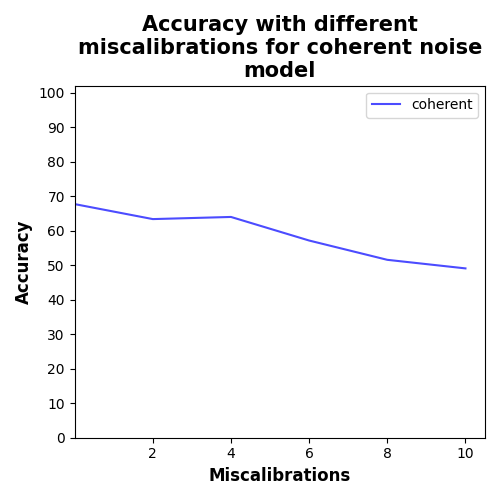
\includegraphics[width=\linewidth]{figures/evaluation_results/diabetes/pqc/figures/accuracy-coherent.png}
      \subcaption{Coherent noise model's accuracy.}
      \label{fig:diabetes1}
  \end{subfigure} \qquad
  \begin{subfigure}{0.45\textwidth}
      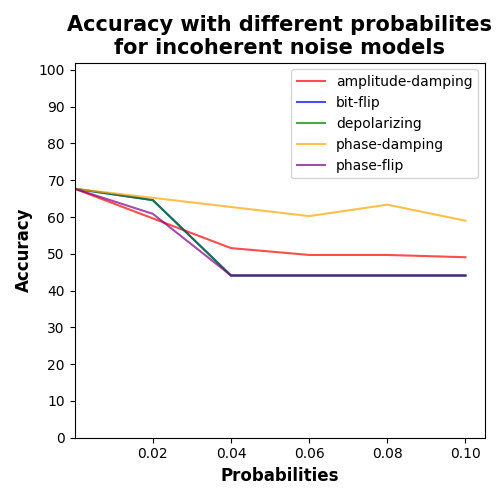
\includegraphics[width=\linewidth]{figures/evaluation_results/diabetes/pqc/figures/accuracy-incoherent.png}
      \subcaption{Incoherent noise models' accuracy.}
      \label{fig:diabetes2}
  \end{subfigure}

  \caption{\ac{vqa}'s accuracy on the \ac{pid} clean test dataset.}
  \label{fig:diabetes-12}
\end{figure} \

\subsection{Adversarial Accuracy}\label{subsection:diabetes-adv-acc} \

In Figure~\ref{fig:diabetes-34} we introduce the effects of the
adversarial attacks on the accuracy of the noiseless \ac{qml}
model. As expected, we can observe that for both adversarial
techniques the performance of the model decreases with increasing
attack strength. For both of the adversarial techniques
we notice a stark accuracy decrease until it stabilizes to around
\(33\%\) after \(0.3\) attack strength. That \ac{fgsm} (Subfig.
~\ref{fig:diabetes3}) has the same performance impact as \ac{pgd}
(Subfigure~\ref{fig:diabetes4}) is not expected, as \ac{fgsm}'s
perturbations tend to be bigger in magnitude and more disruptive
to the input. \

\begin{figure}[!h]
  \centering

  \begin{subfigure}{0.45\textwidth}
      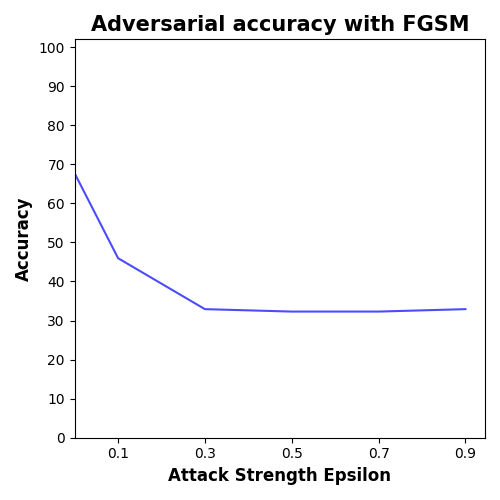
\includegraphics[width=\linewidth]{figures/evaluation_results/diabetes/pqc/figures/none-fgsm.png}
      \subcaption{Noiseless model's \ac{fgsm} adversarial accuracy.}
      \label{fig:diabetes3}
  \end{subfigure} \qquad
  \begin{subfigure}{0.45\textwidth}
      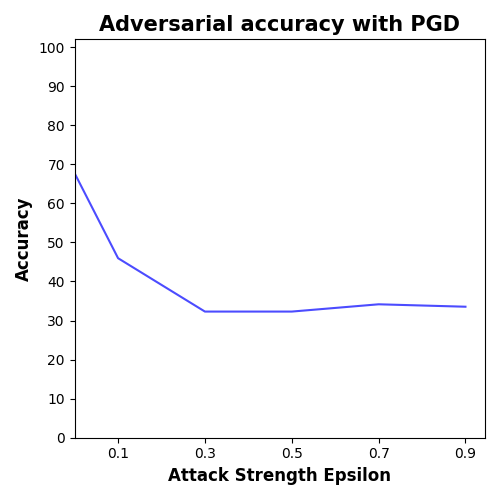
\includegraphics[width=\linewidth]{figures/evaluation_results/diabetes/pqc/figures/none-pgd.png}
      \subcaption{Noiseless model's \ac{pgd} adversarial accuracy.}
      \label{fig:diabetes4}
  \end{subfigure}

  \caption{\ac{vqa}'s accuracy on the adversarial \ac{pid} test dataset.}
  \label{fig:diabetes-34}
\end{figure} \

\subsection{Noisy Models Adversarial Accuracy}\label{subsection:diabetes-noisy-adv-acc} \

In this subsection we introduce the results from performing
the adversarial attacks on the noisy models with different noise
magnitudes for the \ac{pid} dataset. In each graph the color gray
represents the baseline adversarial accuracy obtained by the
noiseless model. \

In Figure~\ref{fig:diabetes-56} we present the outcomes from the amplitude
damping noisy models evaluation. For \ac{fgsm} in Subfigure~\ref{fig:diabetes5}
we note that almost all the noisy models perform equal or better than the
baseline noiseless model after an attack strength of 0.1. Moreover,
a relationship between the magnitude of the noise probability and
the adversarial accuracy can be observed. We notice that the adversarial
accuracy obtains a higher value with models that have a higher noise
probability. The models with 8\% and 10\% noise probability perform
the best, obtaining around 60\% adversarial accuracy at the highest attack
strength of 0.9. This performance is close to the baseline noiseless
performance of 67\% without any attack performed, and is significantly
higher than the noiseless model's adversarial accuracy of around 33\%
at attack strength 0.9. \

\begin{figure}[!h]
  \centering

  \begin{subfigure}{0.45\textwidth}
      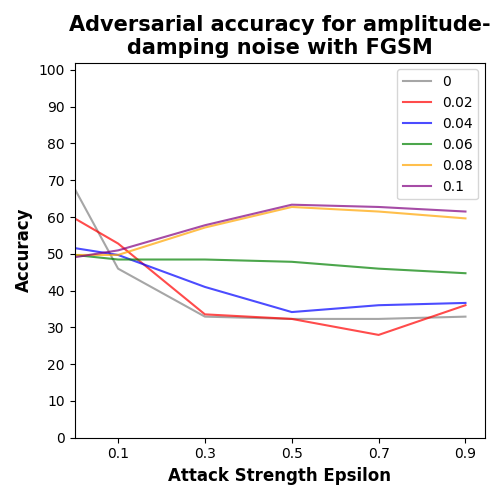
\includegraphics[width=\linewidth]{figures/evaluation_results/diabetes/pqc/figures/amplitude-damping-fgsm.png}
      \subcaption{Amplitude damping noise model's \ac{fgsm} adversarial accuracy.}
      \label{fig:diabetes5}
  \end{subfigure} \qquad
  \begin{subfigure}{0.45\textwidth}
      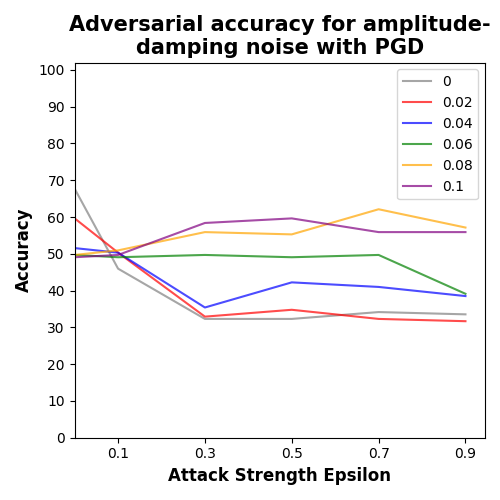
\includegraphics[width=\linewidth]{figures/evaluation_results/diabetes/pqc/figures/amplitude-damping-pgd.png}
      \subcaption{Amplitude damping noise model's \ac{pgd} adversarial accuracy.}
      \label{fig:diabetes6}
  \end{subfigure}
  \caption{Amplitude damping noise models' accuracy on the adversarial \ac{pid} test dataset.}
  \label{fig:diabetes-56}
\end{figure} \

In Subfigure~\ref{fig:diabetes6} we introduce the results from the \ac{pgd}
attack on the amplitude damping noisy models. Similar to the results
obtained from the \ac{fgsm} attack evaluation, we can also observe
a direct link between noise probability and model robustness.
The best performing models are again the models with the highest noise
probability, outperforming the noiseless model by a significant margin.
The models with 8\% and 10\% noise probability achieve an adversarial
accuracy of around 57\% and 56\% respectively at an attack strengths of
0.9. These adversarial accuracy values surpass the performance of
the noiseless model by approximately 24\%. The noisy model with the
worst performance has a 2\% noise probability and performs relatively
equal to the noiseless model, meaning that there is no disadvantage
provoked by any noise appearance with regards to adversarial accuracy. \

In Figure~\ref{fig:diabetes-78} we present the outcomes from the bit-flip
noisy models evaluation. For \ac{fgsm} in Subfigure~\ref{fig:diabetes7}
we note that all of the noisy models except the model with the lowest
noise probability of 2\% behave almost identically throughout all the
attack strength spectrum, obtaining the same higher adversarial
accuracy. These models achieve an adversarial accuracy of around 56\% at
the 0.9 attack strength. While these models have a higher adversarial
accuracy than the noiseless model, the model robustness does not linearly
scale. This means that the model robustness does not increase the
higher the noise probability affecting the model is. The model with
2\% noise probability behaves exactly as the noiseless model, reaching
an adversarial accuracy of around 35\% at an attack strength of 0.9. \

\begin{figure}[!h]
  \centering

  \begin{subfigure}{0.45\textwidth}
      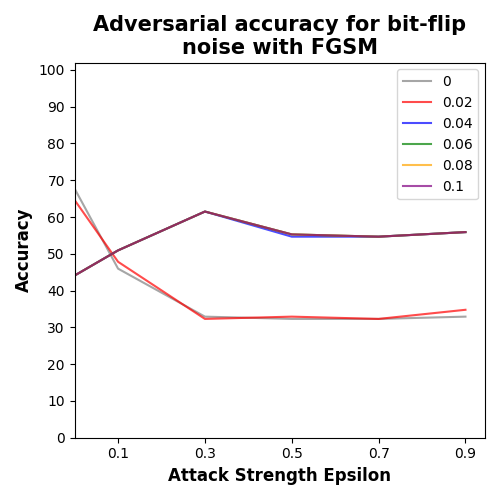
\includegraphics[width=\linewidth]{figures/evaluation_results/diabetes/pqc/figures/bit-flip-fgsm.png}
      \subcaption{Bit-Flip noise model's \ac{fgsm} adversarial accuracy.}
      \label{fig:diabetes7}
  \end{subfigure} \qquad
  \begin{subfigure}{0.45\textwidth}
      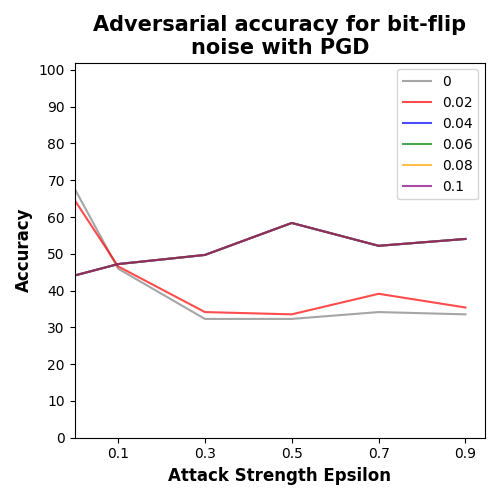
\includegraphics[width=\linewidth]{figures/evaluation_results/diabetes/pqc/figures/bit-flip-pgd.png}
      \subcaption{Bit-Flip noise model's \ac{pgd} adversarial accuracy.}
      \label{fig:diabetes8}
  \end{subfigure}
  \caption{Bit-Flip noise models' accuracy on the adversarial \ac{pid} test dataset.}
  \label{fig:diabetes-78}
\end{figure} \

In Subfigure~\ref{fig:diabetes8} we introduce the results from the \ac{pgd}
attack on the bit-flip noisy models. Analogous to the results obtained
from the \ac{fgsm} attacks, all the noisy models but the model with 2\%
noise probability perform exactly the same. We observe a better model
robustness for the previously mentioned models, achieving a better
adversarial accuracy throughout the attack strength range after 0.1.
These models obtain an adversarial accuracy of around 54\% at
an attack strength of 0.9, higher than the noiseless model's adversarial
accuracy of 33\% at the same attack strength. Nevertheless, the
relationship between model robustness and noise probability magnitude
is not linear. Finally, the model with 2\% noise probability mimics
the noiseless adversarial performance and is lower than the noisier
models. \

In Figure~\ref{fig:diabetes-910} we present the outcomes from the coherent
noisy models evaluation. For \ac{fgsm} in Subfigure~\ref{fig:diabetes9}
we note that the most robust model at the highest attack strength
is the model with a misconfiguration degree of 10. This model obtains
an adversarial accuracy of around 57\% at an attack strength of 0.9. The
worst performing models are the two models with the lowest misconfiguration.
Both models (2 and 4 degree misconfiguration) behave similarly to the
noiseless model, getting an adversarial accuracy of around 35\%. Furthermore,
the model with a 6 degree misconfiguration performs slightly better than
the 8 degree model, but their adversarial accuracy is around 50\% at the
highest attack strength. However, their performance is lower than the
model miscalibrated by 10 degrees. Because of this, we can deduce a
positive relationship between the model robustness and the degree of
misconfiguration. \

\begin{figure}[!h]
  \centering

  \begin{subfigure}{0.45\textwidth}
      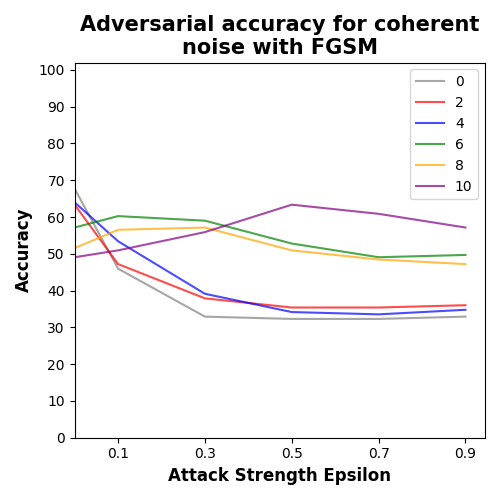
\includegraphics[width=\linewidth]{figures/evaluation_results/diabetes/pqc/figures/coherent-fgsm.png}
      \subcaption{Coherent noise model's \ac{fgsm} adversarial accuracy.}
      \label{fig:diabetes9}
  \end{subfigure} \qquad
  \begin{subfigure}{0.45\textwidth}
      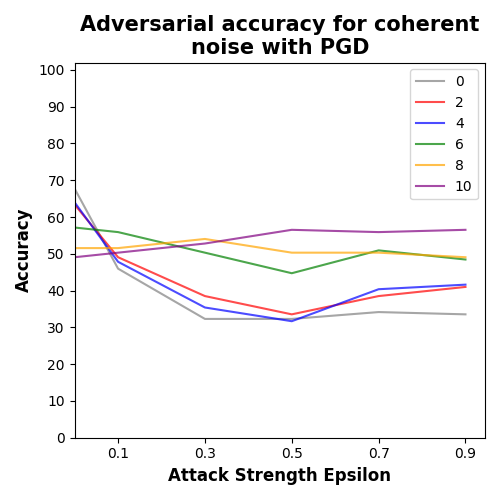
\includegraphics[width=\linewidth]{figures/evaluation_results/diabetes/pqc/figures/coherent-pgd.png}
      \subcaption{Coherent noise model's \ac{pgd} adversarial accuracy.}
      \label{fig:diabetes10}
  \end{subfigure}
  \caption{Coherent noise models' accuracy on the adversarial \ac{pid} test dataset.}
  \label{fig:diabetes-910}
\end{figure} \

In Subfigure~\ref{fig:diabetes10} we introduce the results from the \ac{pgd}
attack on the coherent noisy models. Comparable to the results obtained
from the \ac{fgsm} attack, the noisiest model (10°) has the highest adversarial
accuracy (around 57\%) at the highest attack strength (0.9). The next best
models are the models with a miscalibration of 6 and 8 degrees, they both
achieve around 49\%. Finally, the noisy models with the lowest misconfiguration
degree (2 and 4) perform bettern than the noiseless model. These noisy models
behave similar and get an adversarial accuracy of around 41\%, higher than
the noiseless model's 33\%. Analogous to the results from the \ac{fgsm}
attack, we can derive a positive relationship between the miscalibration
degree and the model robustness at the higher range of the attack strengths
spectrum.  \

In Figure~\ref{fig:diabetes-1112} we present the outcomes from the depolarizing
noisy models evaluation. For \ac{fgsm} in Subfigure~\ref{fig:diabetes11}
we note that the models behave similarly to models with bit-flip noise.
We observe again that the worst performing noisy model is the model with
the lowest noise probability (2\%) and it matches the performance of the
noiseless model. All the remaining noisy models obtain the same accuracy
throughtout the attack strength spectrum and achieve an adversarial
accuracy of around 56\% at 0.9 attack strength. While the results indicate
that a higher noise probability leads to a more robust model, this
relationship does not linearly scale. \

\begin{figure}[!h]
  \centering

  \begin{subfigure}{0.45\textwidth}
      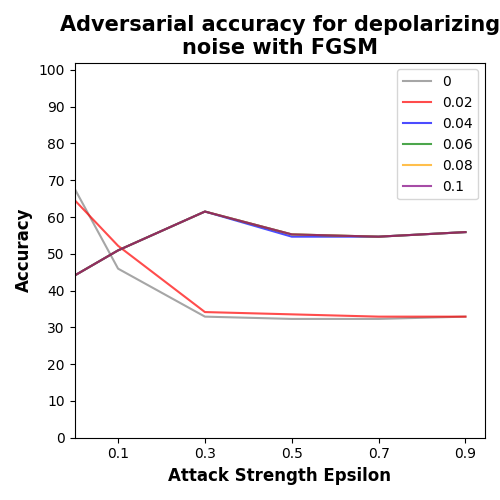
\includegraphics[width=\linewidth]{figures/evaluation_results/diabetes/pqc/figures/depolarizing-fgsm.png}
      \subcaption{Depolarizing noise model's \ac{fgsm} adversarial accuracy.}
      \label{fig:diabetes11}
  \end{subfigure} \qquad
  \begin{subfigure}{0.45\textwidth}
      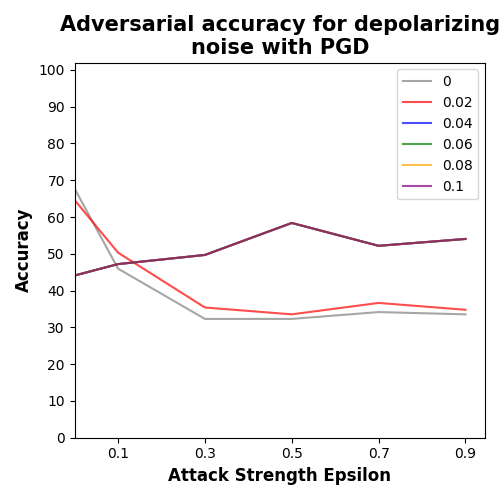
\includegraphics[width=\linewidth]{figures/evaluation_results/diabetes/pqc/figures/depolarizing-pgd.png}
      \subcaption{Depolarizing noise model's \ac{pgd} adversarial accuracy.}
      \label{fig:diabetes12}
  \end{subfigure}
  \caption{Depolarizing noise models' accuracy on the adversarial \ac{pid} test dataset.}
  \label{fig:diabetes-1112}
\end{figure} \

In Subfigure~\ref{fig:diabetes12} we introduce the results from the \ac{pgd}
attack on the depolarizing noisy models. Similar to the results obtaining
from the \ac{fgsm} attack and the evaluation from the noisy bit-flip models,
the worst performing noisy model is the model with the lowest (2\%)
noise probability. This model's performance matches the behavior of the
noiseless model throught the attack strengths range and achives an
adversarial accuracy of around 34\%. The remaining noisy models perfom
similarly throughout the whole attack strength spectrum and obtain
an adversarial accuracy of around 54\% at the highest attack strength
0f 0.9. In this case, a higher noise probability does mean a more robust
model. However, this relationship doesn't scale linearly and robustness
simply increases to a determined adversarial accuracy with a noisy
probability higher than 2\%. \

In Figure~\ref{fig:diabetes-1314} we present the outcomes from the phase damping
noisy models evaluation. For \ac{fgsm} in Subfigure~\ref{fig:diabetes13}
we note that in this case the noiseless and the noisy models have the
same performance throughtout the whole attack strengths, disregarding
the noise probabilities. All the models' adversarial accuracies decrease
significantly to around 35\% at attack strength 0.3 and stabilizes to the
same value at attack strength 0.9. There are some slight variations in
between the models but they are less than 5\% throughout the different
attack strength values. \

\begin{figure}[!h]
  \centering

  \begin{subfigure}{0.45\textwidth}
      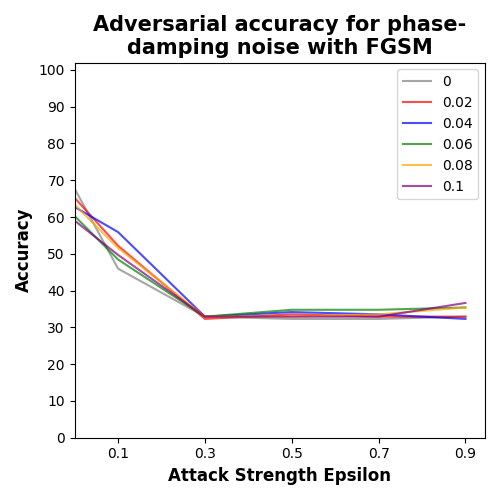
\includegraphics[width=\linewidth]{figures/evaluation_results/diabetes/pqc/figures/phase-damping-fgsm.png}
      \subcaption{Phase Damping noise model's \ac{fgsm} adversarial accuracy.}
      \label{fig:diabetes13}
  \end{subfigure} \qquad
  \begin{subfigure}{0.45\textwidth}
      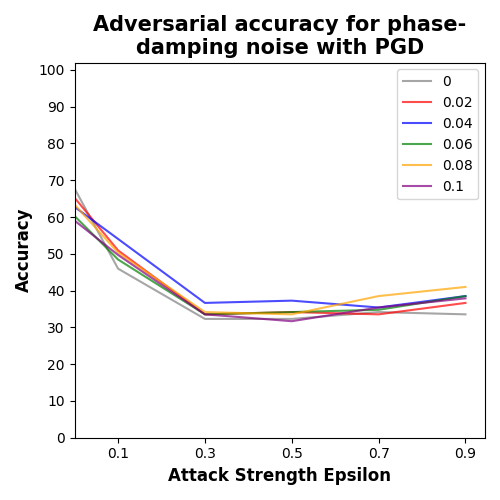
\includegraphics[width=\linewidth]{figures/evaluation_results/diabetes/pqc/figures/phase-damping-pgd.png}
      \subcaption{Phase Damping noise model's \ac{pgd} adversarial accuracy.}
      \label{fig:diabetes14}
  \end{subfigure}
  \caption{Phase damping models' accuracy on the adversarial \ac{pid} test dataset.}
  \label{fig:diabetes-1314}
\end{figure} \

In Subfigure~\ref{fig:diabetes14} we introduce the results from the \ac{pgd}
attack on the phase damping noisy models. These outcomes highly resemble
the values obtained by the \ac{fgsm} attack evaluation. We notice that
all the models (noisy and noiseless) behave similarly throughtout the
range of attack strengths. This means that for phase damping noisy models
the model robustness is independent from the magnitude of the noise
probability. While some slight differences between the adversarial
accuracies from distinct models can be found, the differences are
mostly smaller than 5\% and do not deviate much from the trend set
by all the models. \

In Figure~\ref{fig:diabetes-1516} we present the outcomes from the phase-flip
noisy models evaluation. For \ac{fgsm} in Subfigure~\ref{fig:diabetes15}
we note that the behavior from the bit-flip and depolarizing noisy models
is replicated with phase-flip noise. We can observe that the worst
performing noisy model has 2\% noise probability and matches the noiseless
baseline performance throughout the whole attack strength range. Both 
models obtain around 33\% adversarial accuracy at 0.9 attack strength.
Regarding the remaining noisy models, they all behave similarly across
the attack strength spectrum and they reach an adversarial accuracy at
0.9 attack strength of around 56\%. While no linear relationship between noise
probability and model robustness can be drawn, models with higher noise
probability than 2\% are more robust after an attack strength of 0.1. \

\begin{figure}[!h]
  \centering

  \begin{subfigure}{0.45\textwidth}
      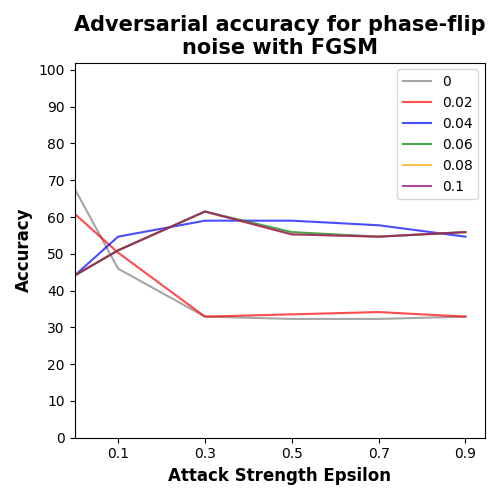
\includegraphics[width=\linewidth]{figures/evaluation_results/diabetes/pqc/figures/phase-flip-fgsm.png}
      \subcaption{Phase-Flip noise model's \ac{fgsm} adversarial accuracy.}
      \label{fig:diabetes15}
  \end{subfigure} \qquad
  \begin{subfigure}{0.45\textwidth}
      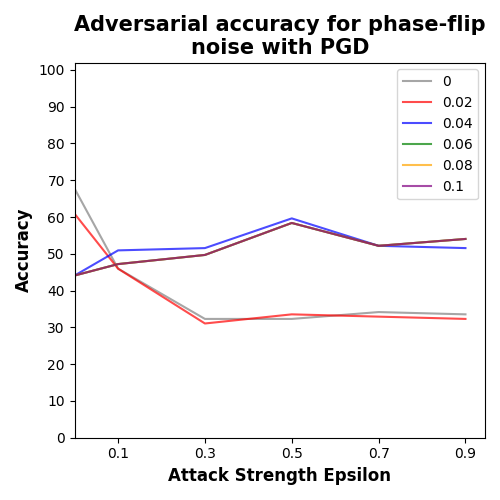
\includegraphics[width=\linewidth]{figures/evaluation_results/diabetes/pqc/figures/phase-flip-pgd.png}
      \subcaption{Phase-Flip noise model's \ac{pgd} adversarial accuracy.}
      \label{fig:diabetes16}
  \end{subfigure}

  \caption{Phase-Flip noise models' accuracy on the adversarial \ac{pid} test dataset.}
  \label{fig:diabetes-1516}
\end{figure} \

In Subfigure~\ref{fig:diabetes16} we introduce the results from the \ac{pgd}
attack on the phase-flip noisy models. The obtained adversarial accuracy
values are comparable to the results obtained in the \ac{fgsm} attacks.
In this case, the noisy models that have a noise probability higher than
2\% are more robust than the remaining models after an attack
strength value of 0.1. The noisy robust models maintain around 50\%
adversarial accuracy throughout the attack strength range and there
are no significant differences in between each other. For the noiseless
model, the performance is almost identical to the model with 2\% noise
probability. Both models stabilize to an adversarial accuracy of around
33\% with an attack strength equal or higher tha 0.3. While no linear
relationship between noise probability and model robustness can be
determined, models with noise probability higher than 2\% perform
significantly better. \

\section{Breast Cancer Dataset}\label{section:breast-cancer-eval} \

The results obtained from training the noisy and noiseless
\ac{qml} models on the Wisconsin Breast Cancer dataset can be found in Subsection
~\ref{subsection:breast-cancer-noisy-acc}. Moreover, the outcomes
of both adversarial attacks will be presented in Subsection
~\ref{subsection:breast-cancer-adv-acc}. Finally, the evaluation
of the noisy models against the adversarial attacks can
are presented in Subsection~\ref{subsection:breast-cancer-noisy-adv-acc}. \

\subsection{Noisy Models Accuracy}\label{subsection:breast-cancer-noisy-acc} \

In Figure~\ref{fig:bc-12} we can observe the results
from the training of noiseless and noisy \ac{qml} models
for the Wisconsin Breast Cancer test dataset. The noiseless baseline model accuracy
can be found on both graphs at the y-intercept, which in
this case is of 84.4\%. Analogous to the \ac{pid} dataset, we note
in Subfigure~\ref{fig:bc1} that for the Wisconsin Breast Cancer
dataset the model accuracy decreases when training
with an increasing coherent noise effect. The model performance
is slowly reduced until it reaches 55.5\% accuracy. \

For incoherent noise models in Subfigure~\ref{fig:bc2}
we can observe a decrease in model accuracy for all the noise
models. In this case, similar to the results from the \ac{pid}
dataset, phase damping noise performs the best of any noise
models. Its accuracy decreases to around 73\%, which is only
10\% less than the noiseless model. The worst performing model
is the one using amplitude damping noise, this model achieves
only around 46\% accuracy. \

Regarding the bit-flip, depolarizing, and phase-flip noise, the model
performance decreases its accuracy to around 68\% starting at
4\% noise probability and remains at that same value for all
higher noise probabilities. The 4\% noise probability convergence
for these specific models also appears in the \ac{pid} dataset. Still,
it seems that there is not any relation between which type of incoherent noise
is used and the performance of the model. While in the \ac{pid}
dataset (Subfig.~\ref{fig:diabetes2}) the best performing models
were the ones using phase and amplitude damping noise, in the
Wisconsin Breast Cancer dataset phase damping noise has again the
highest accuracy but amplitude damping has the worst performance. \

\begin{figure}[!h]
  \centering

  \begin{subfigure}{0.45\textwidth}
      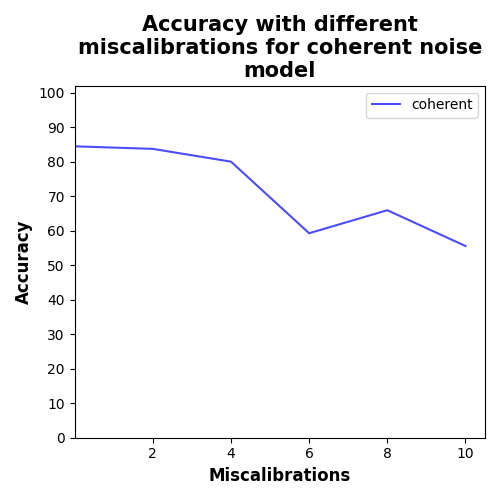
\includegraphics[width=\linewidth]{figures/evaluation_results/breast-cancer/pqc/figures/accuracy-coherent.png}
      \subcaption{Coherent noise model's accuracy.}
      \label{fig:bc1}
  \end{subfigure} \qquad
  \begin{subfigure}{0.45\textwidth}
      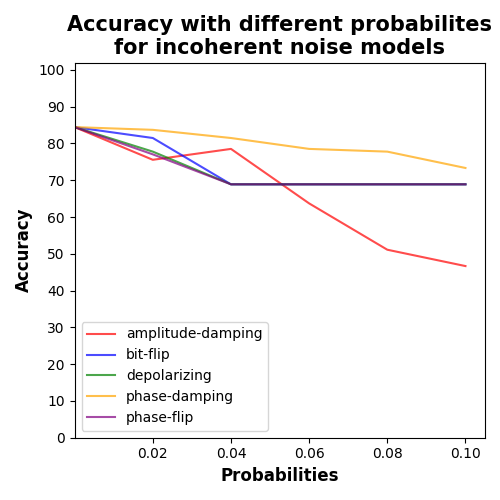
\includegraphics[width=\linewidth]{figures/evaluation_results/breast-cancer/pqc/figures/accuracy-incoherent.png}
      \subcaption{Incoherent noise models' accuracy.}
      \label{fig:bc2}
  \end{subfigure}

  \caption{\ac{vqa}'s accuracy on the Wisconsin Breast Cancer clean test dataset.}
  \label{fig:bc-12}
\end{figure} \

\subsection{Adversarial Accuracy}\label{subsection:breast-cancer-adv-acc} \

In Figure~\ref{fig:bc-34} we introduce the effects of the
adversarial attacks on the accuracy of the noiseless \ac{qml}
model. As expected, we can observe that for both adversarial
techniques the performance of the model decreases with increasing
attack strength. For both of the adversarial techniques
we notice a stark accuracy decrease to around 18\% for \ac{fgsm}
and 29\% for \ac{pgd} at 0.9 attack strength. The \ac{fgsm} technique
(Subfig.~\ref{fig:bc3}) has an overall a lower performance than the
\ac{pgd} attack (Subfigure~\ref{fig:bc4}). This is the expected
behavior, as \ac{fgsm}'s perturbations tend to be bigger in
magnitude and more disruptive to the input. We also note that the
noiseless model's adversarial accuracy for the Wisconsin Breast
Cancer dataset decreases significantly more (around 66\% for
\ac{fgsm} and 55\% for \ac{pgd}) than for the previous datasets. \

\begin{figure}[!h]
  \centering

  \begin{subfigure}{0.45\textwidth}
      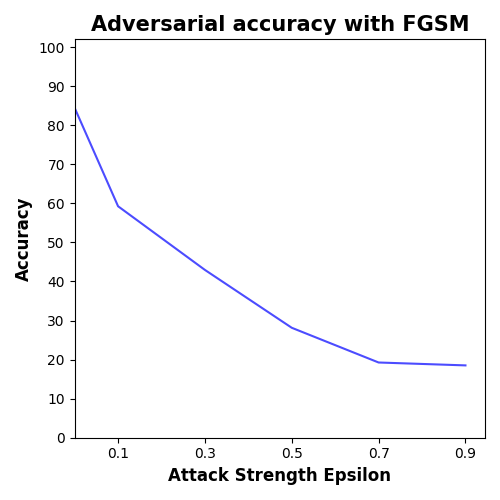
\includegraphics[width=\linewidth]{figures/evaluation_results/breast-cancer/pqc/figures/none-fgsm.png}
      \subcaption{Noiseless model's \ac{fgsm} adversarial accuracy.}
      \label{fig:bc3}
  \end{subfigure} \qquad
  \begin{subfigure}{0.45\textwidth}
      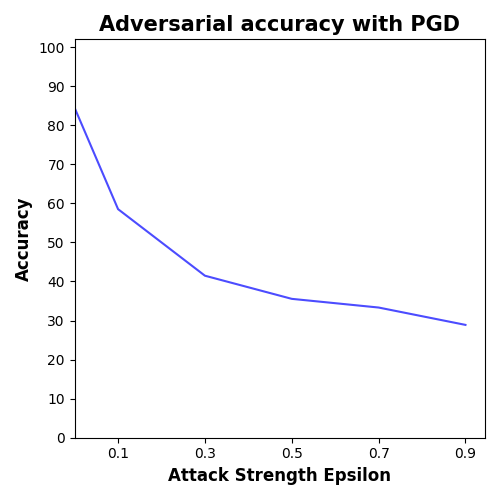
\includegraphics[width=\linewidth]{figures/evaluation_results/breast-cancer/pqc/figures/none-pgd.png}
      \subcaption{Noiseless model's \ac{pgd} adversarial accuracy.}
      \label{fig:bc4}
  \end{subfigure}

  \caption{\ac{vqa}'s accuracy on the adversarial Wisconsin Breast Cancer test dataset.}
  \label{fig:bc-34}
\end{figure} \

\subsection{Noisy Models Adversarial Accuracy}\label{subsection:breast-cancer-noisy-adv-acc} \

In this subsection we introduce the results from performing
the adversarial attacks on the noisy models with different noise
magnitudes for the Wisconsin Breast Cancer dataset. In each graph
the color gray represents the baseline adversarial accuracy obtained
by the noiseless model. \

In Figure~\ref{fig:bc-56} we present the outcomes from the amplitude
damping noisy models evaluation. For \ac{fgsm} in Subfigure~\ref{fig:bc5}
we note that \

\begin{figure}[!h]
  \centering

  \begin{subfigure}{0.45\textwidth}
      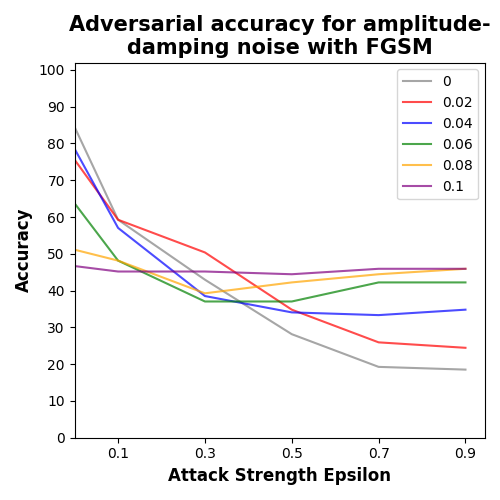
\includegraphics[width=\linewidth]{figures/evaluation_results/breast-cancer/pqc/figures/amplitude-damping-fgsm.png}
      \subcaption{Amplitude damping noise model's \ac{fgsm} adversarial accuracy.}
      \label{fig:bc5}
  \end{subfigure} \qquad
  \begin{subfigure}{0.45\textwidth}
      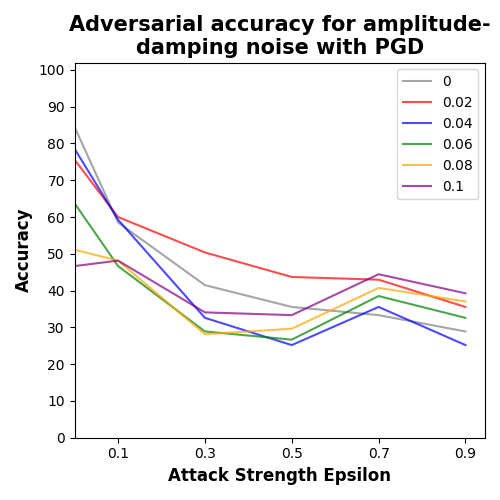
\includegraphics[width=\linewidth]{figures/evaluation_results/breast-cancer/pqc/figures/amplitude-damping-pgd.png}
      \subcaption{Amplitude damping noise model's \ac{pgd} adversarial accuracy.}
      \label{fig:bc6}
  \end{subfigure}
  \caption{Amplitude damping noise models' accuracy on the adversarial Wisconsin Breast Cancer test dataset.}
  \label{fig:bc-56}
\end{figure} \

In Subfigure~\ref{fig:bc6} we introduce the results from the \ac{pgd}
attack on the amplitude damping noisy models. \

In Figure~\ref{fig:bc-78} we present the outcomes from the bit-flip
noisy models evaluation. For \ac{fgsm} in Subfigure~\ref{fig:bc7}
we note that \

\begin{figure}[!h]
  \centering

  \begin{subfigure}{0.45\textwidth}
      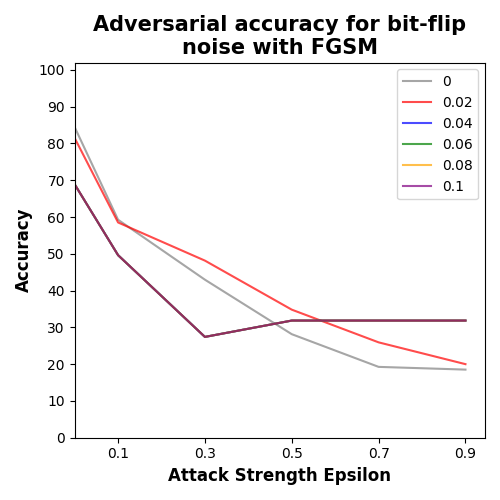
\includegraphics[width=\linewidth]{figures/evaluation_results/breast-cancer/pqc/figures/bit-flip-fgsm.png}
      \subcaption{Bit-Flip noise model's \ac{fgsm} adversarial accuracy.}
      \label{fig:bc7}
  \end{subfigure} \qquad
  \begin{subfigure}{0.45\textwidth}
      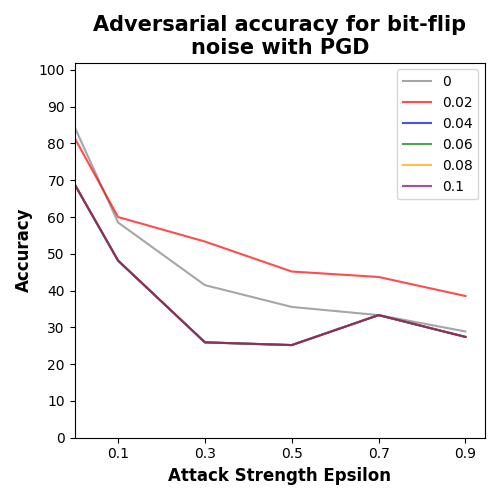
\includegraphics[width=\linewidth]{figures/evaluation_results/breast-cancer/pqc/figures/bit-flip-pgd.png}
      \subcaption{Bit-Flip noise model's \ac{pgd} adversarial accuracy.}
      \label{fig:bc8}
  \end{subfigure}
  \caption{Bit-Flip noise models' accuracy on the adversarial Wisconsin Breast Cancer test dataset.}
  \label{fig:bc-78}
\end{figure} \

In Subfigure~\ref{fig:bc8} we introduce the results from the \ac{pgd}
attack on the bit-flip noisy models. \

In Figure~\ref{fig:bc-910} we present the outcomes from the coherent
noisy models evaluation. For \ac{fgsm} in Subfigure~\ref{fig:bc9}
we note that \

\begin{figure}[!h]
  \centering

  \begin{subfigure}{0.45\textwidth}
      \includegraphics[width=\linewidth]{figures/evaluation_results/breast-cancer/pqc/figures/coherent-fgsm.png}
      \subcaption{Coherent noise model's \ac{fgsm} adversarial accuracy.}
      \label{fig:bc9}
  \end{subfigure} \qquad
  \begin{subfigure}{0.45\textwidth}
      \includegraphics[width=\linewidth]{figures/evaluation_results/breast-cancer/pqc/figures/coherent-pgd.png}
      \subcaption{Coherent noise model's \ac{pgd} adversarial accuracy.}
      \label{fig:bc10}
  \end{subfigure}
  \caption{Coherent noise models' accuracy on the adversarial Wisconsin Breast Cancer test dataset.}
  \label{fig:bc-910}
\end{figure} \

In Subfigure~\ref{fig:bc10} we introduce the results from the \ac{pgd}
attack on the coherent noisy models. \

In Figure~\ref{fig:bc-1112} we present the outcomes from the depolarizing
noisy models evaluation. For \ac{fgsm} in Subfigure~\ref{fig:bc11}
we note that \

\begin{figure}[!h]
  \centering

  \begin{subfigure}{0.45\textwidth}
      \includegraphics[width=\linewidth]{figures/evaluation_results/breast-cancer/pqc/figures/depolarizing-fgsm.png}
      \subcaption{Depolarizing noise model's \ac{fgsm} adversarial accuracy.}
      \label{fig:bc11}
  \end{subfigure} \qquad
  \begin{subfigure}{0.45\textwidth}
      \includegraphics[width=\linewidth]{figures/evaluation_results/breast-cancer/pqc/figures/depolarizing-pgd.png}
      \subcaption{Depolarizing noise model's \ac{pgd} adversarial accuracy.}
      \label{fig:bc12}
  \end{subfigure}
  \caption{Depolarizing noise models' accuracy on the adversarial Wisconsin Breast Cancer test dataset.}
  \label{fig:bc-1112}
\end{figure} \

In Subfigure~\ref{fig:bc12} we introduce the results from the \ac{pgd}
attack on the depolarizing noisy models. \

In Figure~\ref{fig:bc-1314} we present the outcomes from the phase damping
noisy models evaluation. For \ac{fgsm} in Subfigure~\ref{fig:bc13}
we note that \

\begin{figure}[!h]
  \centering

  \begin{subfigure}{0.45\textwidth}
      \includegraphics[width=\linewidth]{figures/evaluation_results/breast-cancer/pqc/figures/phase-damping-fgsm.png}
      \subcaption{Phase Damping noise model's \ac{fgsm} adversarial accuracy.}
      \label{fig:bc13}
  \end{subfigure} \qquad
  \begin{subfigure}{0.45\textwidth}
      \includegraphics[width=\linewidth]{figures/evaluation_results/breast-cancer/pqc/figures/phase-damping-pgd.png}
      \subcaption{Phase Damping noise model's \ac{pgd} adversarial accuracy.}
      \label{fig:bc14}
  \end{subfigure}
  \caption{Phase damping models' accuracy on the adversarial Wisconsin Breast Cancer test dataset.}
  \label{fig:bc-1314}
\end{figure} \

In Subfigure~\ref{fig:bc14} we introduce the results from the \ac{pgd}
attack on the phase damping noisy models. \

In Figure~\ref{fig:bc-1516} we present the outcomes from the phase-flip
noisy models evaluation. For \ac{fgsm} in Subfigure~\ref{fig:bc15}
we note that \

\begin{figure}[!h]
  \centering

  \begin{subfigure}{0.45\textwidth}
      \includegraphics[width=\linewidth]{figures/evaluation_results/breast-cancer/pqc/figures/phase-flip-fgsm.png}
      \subcaption{Phase-Flip noise model's \ac{fgsm} adversarial accuracy.}
      \label{fig:bc15}
  \end{subfigure} \qquad
  \begin{subfigure}{0.45\textwidth}
      \includegraphics[width=\linewidth]{figures/evaluation_results/breast-cancer/pqc/figures/phase-flip-pgd.png}
      \subcaption{Phase-Flip noise model's \ac{pgd} adversarial accuracy.}
      \label{fig:bc16}
  \end{subfigure}

  \caption{Phase-Flip noise models' accuracy on the adversarial Wisconsin Breast Cancer test dataset.}
  \label{fig:bc-1516}
\end{figure} \

In Subfigure~\ref{fig:bc16} we introduce the results from the \ac{pgd}
attack on the phase-flip noisy models. \

\section{Plus-Minus Dataset}\label{section:plus-minus-eval} \

\subsection{Noisy Models Accuracy}\label{subsection:plus-minus-noisy-acc} \

\subsection{Adversarial Accuracy}\label{subsection:plus-minus-adv-acc} \

\subsection{Noisy Models Adversarial Accuracy}\label{subsection:plus-minus-noisy-adv-acc} \

\subsection{Discussion}\label{subsection:discussion} \

PGD results might vary as the iterative process will result in different
values every time. \

Iris dataset might be too simple on clean dataset. (probs not if it is being affected by the adversarial attacks)

Coherent noise might just work as a bias term on the clean dataset? \

Iris dataset notes: \

Amplitude damping works worse than baseline, no relation between noise
probability and adv accuracy. \

bit-flip, some models perform better than baseline but no relationship
between noise probability and adv accuracy can be found. \

for pgd with bit-flip and amplitude damping the performance gets better
for some models with increased attack strength. \

coherent noise seems to increase model robustness, specially at higher noise
probabilities, maybe works as a bias term that better enables the model
to adjust the classification threshold. \

depolarizing noise is in general better in both attacks than the baseline
model but no conclusions can be drawns. \

phase-damping: main diff between pgd and fgsm is the accuracy levels,
were fgsm affects reduces more the accuracy than pgd. this applies to
all noisy models, so there isn't a different noisy model behavior
depending on the adv attack, just a change in the adv acc values. \

phase-flip: slight correlation found between noise probs and robustness,
it is an inverse relationship, meaning that the higher the noise the worse
the performance.

Diabetes dataset notes: \

amplitude-damping: higher noise probability leads to more robust models. \

bit-flip: more noise equals more robustness but it doesn't scale linearly \

coherent: same as amplitude-damping noise \

depolarizing:  same as bit-flip \

phase damping: robustness independent from noise \

phase-flip: same as bit-flip and depolarizing \

Breast Cancer dataset notes: \

Adversarial accuracy is significantly lowered, maybe because it has
more features to modify. \


1.	Explain why decoherent noise is used and not coherent. \

  a. Coherent noise will probably just shift the bias. \

  b. Coherent noise might add too much noise (quadratic growth). \

  c. True random noise is required to improve generalization. \

% TODO: Do an experiment implementing coherent noise to prove this claim.
% Use https://pennylane.ai/qml/demos/tutorial_variational_classifier/ - circuit-centric quantum classifier ansatz

\section{Variational Quantum Algorithm Model Accuracy}\label{section:vqa_accuracy} \

% TODO: State the result of training QVC with regards to the chosen datasets.
% TODO: Compare to paper and state why they might be valid results.

\section{Variational Quantum Algorithm Model Adversarial Accuracy}\label{section:vqa_adversarial_accuracy} \

% TODO: Present results per dataset of the different attacks and attack strengths
\chapter{Summary}\label{chapter:summary} \

Summarize worked done and findings. \
\chapter{Future Work}\label{chapter:future_work} \

When creating the weights to be trained, a proper selection might increase the accuracy of the models or avoid barren plateaus. \

Investigate \ac{qml} model training with different optimizers, maybe even no gradient-based methods. \

Investigate the influence of the different loss functions when training a \ac{qml} model. How to interpret correctly the measurements at the end of the \ac{qml} model, can it be assumed to be a probability distribution? \

Do experiments with new ansätze, maybe quantum kernels. \

Do experiments with new encoding mechanisms, angle, etc. (encoding might have a big influence in how the features are interpreted) \

Perform other different attacks like carlini and wagner \

Perform transfer attacks between noisy models including the noiseless models. Basically create adversarial examples from noisy models and see how effective they are against other noisy models or the noiseless model. \

% Take noise out of the evaluation part of the training (i think currently the noisy model is used to calculate the accuracy of the model during training) \
\chapter{Style}\label{chapter:style}

\section{Section}
Citation test~\cite{national_academies_of_sciences_engineering_and_medicine_quantum_2019}.
Acronyms must be added in \texttt{main.tex} and are referenced using macros. The first occurrence is automatically replaced with the long version of the acronym, while all subsequent usages use the abbreviation.

E.g. \texttt{\textbackslash{} ac\{tum\}, \textbackslash{} ac\{tum\}} $\Rightarrow$ \ac{tum}, \ac{tum}

For more details, see the documentation of the \texttt{acronym} package\footnote{\url{https://ctan.org/pkg/acronym}}.
\subsection{Subsection}

See~\autoref{tab:sample}, \autoref{fig:sample-drawing}, \autoref{fig:sample-plot}, \autoref{fig:sample-listing}.

\begin{table}[htpb]
  \caption[Example table]{An example for a simple table.}\label{tab:sample}
  \centering
  \begin{tabular}{l l l l}
    \toprule
      A & B & C & D \\
    \midrule
      1 & 2 & 1 & 2 \\
      2 & 3 & 2 & 3 \\
    \bottomrule
  \end{tabular}
\end{table}

\begin{figure}[htpb]
  \centering
  % This should probably go into a file in figures/
  \begin{tikzpicture}[node distance=3cm]
    \node (R0) {$R_1$};
    \node (R1) [right of=R0] {$R_2$};
    \node (R2) [below of=R1] {$R_4$};
    \node (R3) [below of=R0] {$R_3$};
    \node (R4) [right of=R1] {$R_5$};

    \path[every node]
      (R0) edge (R1)
      (R0) edge (R3)
      (R3) edge (R2)
      (R2) edge (R1)
      (R1) edge (R4);
  \end{tikzpicture}
  \caption[Example drawing]{An example for a simple drawing.}\label{fig:sample-drawing}
\end{figure}

\begin{figure}[htpb]
  \centering

  \pgfplotstableset{col sep=&, row sep=\\}
  % This should probably go into a file in data/
  \pgfplotstableread{
    a & b    \\
    1 & 1000 \\
    2 & 1500 \\
    3 & 1600 \\
  }\exampleA{}
  \pgfplotstableread{
    a & b    \\
    1 & 1200 \\
    2 & 800 \\
    3 & 1400 \\
  }\exampleB{}
  % This should probably go into a file in figures/
  \begin{tikzpicture}
    \begin{axis}[
        ymin=0,
        legend style={legend pos=south east},
        grid,
        thick,
        ylabel=Y,
        xlabel=X
      ]
      \addplot table[x=a, y=b]{\exampleA};
      \addlegendentry{Example A};
      \addplot table[x=a, y=b]{\exampleB};
      \addlegendentry{Example B};
    \end{axis}
  \end{tikzpicture}
  \caption[Example plot]{An example for a simple plot.}\label{fig:sample-plot}
\end{figure}

\begin{figure}[htpb]
  \centering
  \begin{tabular}{c}
  \begin{lstlisting}[language=SQL]
    SELECT * FROM tbl WHERE tbl.str = "str"
  \end{lstlisting}
  \end{tabular}
  \caption[Example listing]{An example for a source code listing.}\label{fig:sample-listing}
\end{figure}


%\appendix
%\chapter{Dataset Graphs}\label{chapter:appendix-iris} \

\begin{figure}[!b]
    \centering

    \begin{subfigure}{0.40\textwidth}
        \includegraphics[width=\linewidth]{figures/accuracy-graph.png}
        \subcaption{1}
        \label{fig:arm1}
    \end{subfigure}
    \begin{subfigure}{0.40\textwidth}
        \includegraphics[width=\linewidth]{figures/accuracy-graph.png}
        \subcaption{2}
        \label{fig:arm2}
    \end{subfigure}

\medskip

    \begin{subfigure}{0.40\textwidth}
        \includegraphics[width=\linewidth]{figures/accuracy-graph.png}
        \subcaption{3}
        \label{fig:arm3}
    \end{subfigure}
    \begin{subfigure}{0.40\textwidth}
        \includegraphics[width=\linewidth]{figures/accuracy-graph.png}
        \subcaption{4}
        \label{fig:arm4}
    \end{subfigure}

    \caption{graphs big caption}
\end{figure}

\begin{figure}[!b]\ContinuedFloat
    \centering

    \begin{subfigure}{0.39\textwidth}
        \includegraphics[width=\linewidth]{figures/accuracy-graph.png}
        \subcaption{5}
        \label{fig:arm5}
    \end{subfigure}
    \begin{subfigure}{0.39\textwidth}
        \includegraphics[width=\linewidth]{figures/accuracy-graph.png}
        \subcaption{6}
        \label{fig:arm6}
    \end{subfigure}

    \medskip

    \begin{subfigure}{0.39\textwidth}
        \includegraphics[width=\linewidth]{figures/accuracy-graph.png}
        \subcaption{7}
        \label{fig:arm7}
    \end{subfigure}
    \begin{subfigure}{0.39\textwidth}
        \includegraphics[width=\linewidth]{figures/accuracy-graph.png}
        \subcaption{8}
        \label{fig:arm8}
    \end{subfigure}

    \medskip
    
    \begin{subfigure}{0.39\textwidth}
        \includegraphics[width=\linewidth]{figures/accuracy-graph.png}
        \subcaption{9}
        \label{fig:arm9}
    \end{subfigure}
    \begin{subfigure}{0.39\textwidth}
        \includegraphics[width=\linewidth]{figures/accuracy-graph.png}
        \subcaption{10}
        \label{fig:arm10}
    \end{subfigure}

    \caption{graphs big caption (cont.)}
\end{figure}

\begin{figure}[!b]\ContinuedFloat
    \centering

    \begin{subfigure}{0.39\textwidth}
        \includegraphics[width=\linewidth]{figures/accuracy-graph.png}
        \subcaption{11}
        \label{fig:arm11}
    \end{subfigure}
    \begin{subfigure}{0.39\textwidth}
        \includegraphics[width=\linewidth]{figures/accuracy-graph.png}
        \subcaption{12}
        \label{fig:arm12}
    \end{subfigure}

    \medskip

    \begin{subfigure}{0.39\textwidth}
        \includegraphics[width=\linewidth]{figures/accuracy-graph.png}
        \subcaption{13}
        \label{fig:arm13}
    \end{subfigure}
    \begin{subfigure}{0.39\textwidth}
        \includegraphics[width=\linewidth]{figures/accuracy-graph.png}
        \subcaption{14}
        \label{fig:arm14}
    \end{subfigure}

    \medskip
    
    \begin{subfigure}{0.39\textwidth}
        \includegraphics[width=\linewidth]{figures/accuracy-graph.png}
        \subcaption{15}
        \label{fig:arm15}
    \end{subfigure}
    \begin{subfigure}{0.39\textwidth}
        \includegraphics[width=\linewidth]{figures/accuracy-graph.png}
        \subcaption{16}
        \label{fig:arm16}
    \end{subfigure}

    \caption{graphs big caption (cont.)}
\end{figure}

\microtypesetup{protrusion=false}

\addchap{Abbreviations}
\begin{acronym}
	\itemsep-.25\baselineskip{}
	\acro{tum}[TUM]{Technical University of Munich}
	\acro{nisq}[NISQ]{Noisy Intermediate-Scale Quantum}
	\acro{ml}[ML]{Machine Learning}
	\acro{qml}[QML]{Quantum Machine Learning}
	\acro{cnot}[CNOT]{Controlled NOT}
	\acro{pid}[PID]{Pima Indians Diabetes}
	\acro{vqa}[VQA]{Variational Quantum Algorithm}
	\acro{aml}[AML]{Adversarial Machine Learning}
	\acro{fgsm}[FGSM]{Fast Gradient Sign Method}
	\acro{pgd}[PGD]{Projected Gradient Descent}
	% TODO: add acronyms
\end{acronym}

\listoffigures{}
\listoftables{}
\microtypesetup{protrusion=true}
\printbibliography{}

\end{document}
